\documentclass[11pt,a4paper,twoside]{article}
\usepackage{package/lmuthesis}

\prof{Prof.\ Dr.\ Heinrich Hu{\ss}mann}
\title{Understanding and Predicting\\Web Browsing Behavior}
\author{Changkun Ou}
\email{hi@changkun.us}
\bearbeitungszeitraum{12.8.2018 bis 12.2.2019}
\betreuer{Malin Eiband and Dr. Daniel Buschek}
\aufgabenstellung{
    \begin{description}
        \item[Understanding and Predicting User Browsing Behavior]
 
        \item[Problem Statement] To be added
        % Under standing user behavior helps designer optimize 
        % their product user experiences. Meanwhile, users can benefit more productive 
        % from it. Since user intents are elusive, changeable and sometimes even undetermined, 
        % predict their behavior usually difficult and impoissible. In most cases, a user may 
        % performs a series of wasted actions before reach an intent destination. 
        % Nevertheless, user intents becomes clear step by step after performs a series of 
        % actions in a given context. 
        \item[Scope of the Thesis] To be added
        % To tackle the aforementioned challenges, the objective of this thesis is to develop a system that tracking user actions within a website, 
        % As a first step, literature review ...
        % Based on the literature review, a intent model should be developed ...
        % Then a system should implements the ...
        % Nevertheless, user intents becomes clear step by step after performs a series of actions in a given context. 
        \item[Tasks] (1) Conduct a literature review to identify research questions regarding
        clickstream research that are of interest to researchers and practitioners \\
        (2) Design a machine learning based model in clickstream modeling and 
        creating an appropriate experiment with theoretical support to justify model performance and its interpretability \\
        (3) Develop an web application as a demonstration of the model and evolving it as a generic architecture
        for the proposed model.
        \item[Requirements] Strong skills in mathematical modeling and machine learning approaches, independent scientific work and creative problem solving,
        industrial experience in web development and architecting.
        %asdfasdf
        \item[Keywords] Clickstream, User Browsing Behavior, Machine Learning, Web
    \end{description}
}
\acknoledgement{
    I would like to appreciate Malin Eiband and Dr. Daniel Buschek for many of their great and 
    constructive discussions, suggestion around thesis topic selection, model statements,
    thesis structuring as well as their pacient of given supervision to the thesis. 
    The thesis would not be accomplished without them. Afterward, I am full of gratitude to 
    Prof. Hussmann and Prof. Butz for offering me an unexpected opportunity to study aboard in Germany 
    as well as their kindly helps regarding study and living in my academic period.
    Next, I wish to thank my best friend Yi, schoolfellow Yifei and Xingying, 
    and former colleague Jin for their inspiring discussions surrounding my thesis. 
    Finally, I will forever be beholden to my parents for their continuous supports 
    while my postgraduate study, since they dedicated their live to my better future.
}
\abstract{
Clickstream applications appeared at the end of last century and 
have proliferated the heart of our Internet world.
Trades, public opinions, and almost every trace of web requests are precisely recorded 
on server-side log files.
The fundamental interaction between a web service client and server stands immutably, 
despite the fact that mobile devices have governed our daily life.
In this thesis, we propose a machine learning model that characterizes user browsing behavior 
while involving multi-tab branching and backtrack actions in a browser instead of
web request-based clickstreams. We call it the Action Path model.
To justify our model, we first established a lab study and collected individuals' clickstream data, 
which consisted of chronologic URLs and corresponding stay durations of each URL
with designed nine different contexts given web browsing tasks for three mainstream websites 
based on the theory of information behavior.
Each website has three types of tasks, including a goal-oriented task, fuzzy task and 
exploring browsing task. They characterize the corresponding three browsing 
behaviors.
By analyzing the subject's trace from our lab study, we seek to archive the following goals:
1) Understanding: identify if browsing behaviors are distinguishable and 
finding common patterns that appear in an action path.
2) Classification: to separate and report browsing behaviors on the web, which help 
users better understanding their status.
3) Prediction: present the future click path more than one step with the given context of
the browsing history in a session.
To achieve these goals, our quantitative analysis indicates that goal-oriented, fuzzy and exploring
browsing behaviors are classifiable with 100.00\% precision based on the combination of 
chronologic URLs and stay duration. 
The prediction performance of our model shows higher than 60\% accuracy for 
3 to 5 steps of future clickstream prediction.
Meanwhile, our qualitative analysis of the clickstream indicates 5 observed patterns, 
including ``ring'',``star'', ``overlap'', ``hesitation'' and ``cluster'' patterns, which 
represent the patterns of an action path. 
As an illustration of application, we also developed a browser plugin that proactively serves users,
as well as suggesting predictions of the possible future user clicks.
Furthermore, a generalized design of our model and plugin communication protocol 
are discussed for possibility of formalizing them as standard Web APIs to help designer and 
developers to improve and monitor the user experience of their products.
To the best of our knowledge, this is the first such detailed study regarding web browsing 
behavior modeling based on client-side collected clickstreams.
}

\begin{document}

\makecover
\makeaufgabenstellung
\makededication
\makeabstract
\maketoc
% \listoffigures
% \listoftables
\cleardoublepage

\section{Introduction}

\subsection{Origin of Clickstream Research}

The word "clickstream" first coined in 1995 \cite{friedman1995}, a media comments article 
introduces a novel concept of tracing cyberlife of users over the nowadays "Internet". 
Afterwards, people realized the potential danger and value of tracing cyberspace, which opens a
large discussion of clickstream influences, such as frequency based mining of clickstream \cite{brodwin1995},
privacy concerns \cite{reidenberg1996governing}, and database schema of such a time series data \cite{courtheoux2000database}.

Privacy discussion concludes collecting traces over net clearly offence the rights of users,
the practice violates the openness and transparency of a service to a user.
Serious criticism arise the tracing becomes a loss of democratic governance \cite{gindin1997lost}.

Technologies is not guilty. After years of discussion, positive opinion proposes the rules 
\cite{reidenberg1996governing} and regulations \cite{skok1999establishing} in cyberspace,
means of protecting information privacy in cyberspace transactions \cite{kang1997information},
and approaches to resolve conflicting international data privacy \cite{reidenberg1999resolving}.

Subsequently, bussiness man agilely responses to the concept and immediately initate 
commercial tracking of their customer to improving marketing affects \cite{novick1995}, 
customer service and precise advertisment\cite{reagle1999platform, bucklin2000sticky}, 
even measuring product success \cite{schonberg2000measuring}.

At the turn of this century, common reviews start accept the technology of clickstream,
clickstream data has confirmed by industrial practice, which opens a new era in 
customer service \cite{walsh2000internet}, most of website users start accept their click path data 
be aggregate analysed on the server side \cite{carr2000hypermediation}.

Clickstream data grows fast and becomes plentiful, researchers start convey the original concept of clickstream,
tracking customer selections, into various applications, such as usability testing \cite{Waterson:2002:LOW:506443.506602},
understanding social network sentiment \cite{Schneider:2009:UOS:1644893.1644899}, and developed visualizing
technique to better interpret clickstream data \cite{Waterson:2002:DTU:1556262.1556276}.

Analysis, reports and characterizing of clickstream gains its popularity, Mobasher et al. \cite{Mobasher:2001:EPB:502932.502935}
suggests personalize user based on association rule from their web usage data. Chatterjee et al. \cite{chatterjee2003modeling} 
first proposed E-commerce websites should use clickstream to tracking customer navigation pattern instead of essential choice, 
associating and binding products for observing responses of a customer.

\subsection{This thesis}

% 讨论 clickstream 的起源,讨论 clickstream 的影响,
% 为什么 clickstream 变得重要,为什么 clickstream 是一个值得研究的类别,
% clickstream 的价值都体现在哪些方面,以前的一些 clickstream 都有些什么内容。

% 大体上介绍本论文想要研究 clickstream 的内容,
% 这包括如何开展 clickstream 数据的搜集工作,搜集任务是什么,主要使用的方法,
% 以及得出的结论。根据这些结论,文章提出了一个客户端的插件,
% 能够在现代浏览器上支持这样的预测,
% 同时还进一步探讨了此项功能作为浏览器内建功能甚至浏览器 API 的可能性。

\cleardoublepage
\section{Related Works}
\label{ch:relate}

% - 讨论 client-side 的 clickstream 为什么值得研究,比较服务端搜集的 clickstream 产生的明显变化是什么。
% - 讨论现有的 client-side clickstream 研究分别是针对什么方向的,他们的结论主要是什么,都有什么样的改进空间。
% - 以前的 clickstream 只有类别级的分配模型,通过人工设计某个特定网站的马尔科夫模型来学习用户在不同类别之间的跳转概率。但当变为客户端后,数据变得更加充分,用户在一段时间内可能不局限于某个特定的网站,同时可能被其他网站干扰。

In this chapter, we discuss the former research that releats to our work, including
the existing approaches to clickstream behavior modeling, the evolution of information 
behavior theory regarding how it adapts to our digital world, as well as the 
most related recent advances regarding sequence learning.

\subsection{Clickstream Behavior Modeling}

Clickstream behavior research can be traced back to the year when the word ``clickstream''
was invented. Eearly clickstream behavior research studied the navigational behavior
of user \cite{mandese1995clickstreams, brodwin1995} and 
they binary classified clickstream based on the degree of linearity.

Mobasher et al. discovered the effective and scalable techniques \cite{Mobasher:2001:EPB:502932.502935} for Web personalization
by using association rules and built a recommondation system. Goldfrab invistigates \cite{goldfarb2002analyzing} 
the website choice behavior based on clickstream data and suggests that clickstream simulate company strategy changes.
Afterwards, 
Chatterjee et al. \cite{chatterjee2003modeling} first conduct 
the previous research regarding clickstream to an actual commercial website.
They found that clickstream represents an implication that dynamic advertising
based on customer clickstream history influence the future clickstream of the customer
and increase the interaction with the dynamic advertisement.
More techniquely, Ting et al. uses common sequences to find unexpected browsing behavior \cite{Ting:2005:UMF:1092358.1092469},
and then use their findings to improve website design. 

The most recent research evolved the approach of clickstream modeling,
Wang et al.\cite{Wang:2016:UCC:2858036.2858107} proposed a unsupervised appraoch to model clickstream without labeling.
Chi et al. proposed an analysis framework \cite{chi2017towards} for the general understanding of online information behavior
in a specific page. However, their framework only fits for server side collected clickstream other than a real user clickstream.
Then, Wang et al. \cite{Wang:2017:CUB:3127338.3068332} improved their unsupervised appraoch,
and summarized more approaches for clickstream behavior modeling that identifies span ad abuse
for a specific website. Park et al. models and detects a behavior change among student while learning 
based on Poisson process \cite{Park:2017:DCS:3027385.3027430} to
help improve online learning experience. Amo et al. \cite{amo2018learning} further visualizes search-stream
behavior based on student clickstream on a class, and Shimada et al. proves \cite{Shimada:2018:OCD:3170358.3170412}
online change detection while monitoring on student behavior is possible based on a sliding window.

Zaloudek gives an review on the comparasion \cite{mastersthesis} traditional method to model clickstream data,
then proposed a principle component analysis based method for a semi-supervised learning
of clickstream data, however their approach does not work well on clustering task, and 
the best performance is obtained by traditional multilayer perceptron algorithm.
Chandramohan and Ravindran then further investigate the neural approach on clicksteam mining \cite{N:2018:NAB:3152494.3152505},
they verified that complexy LSTM with Attention mechanism is able to capture whether a user
is intent to buy a product or not based on server side collected clickstream.
Surprisingly, Gundala and Spezzano \cite{Gundala:2018:RDH:3184558.3191644} simply use a Lasso
regression based on sofisticated feature engineering 
archived AOC score 0.769 for reader demand hyperlink prediction on Wikipedia clickstream dataset.

Kammenhuber et al. is the first study regarding client side clickstream \cite{Kammenhuber:2006:WSC:1177080.1177110}.
They proposed a finite-state Markov model that models user's search behavior on a level of
topic categories. Unfortunately their dataset are collected from network package traffic,
and did not consider the time a user spend in each page.


% 关于 assistent 的研究
% @article{lieberman1995letizia,
%   title={Letizia: An agent that assists web browsing},
%   author={Lieberman, Henry and others},
%   journal={IJCAI (1)},
%   volume={1995},
%   pages={924--929},
%   year={1995}
% }

\begin{figure}[H]
    \centering
    \includegraphics[width=0.55\textwidth]{figures/branching-and-backtracking}
    \caption{Parallel browsing behavior: branching phenomenon \cite{huang2010parallel}}
    \label{fig:backtrace}
\end{figure}

Liu et al. \cite{liu2010understanding} studied a specific user behavior on dwell time on web pages, and concluded that
Weibull distribution is the most appropriate distribution to characterize this behavior. 
Huang et al. \cite{huang2010parallel, huang2012no} further 
noticed the behavior of branching parallel browssing and backtracking browsing
behavior on modern browsers, as shown in Figure \ref{fig:backtrace}, 
and presented an frequent analysis for the distribution of these two behavior individually.

Unfortunately, as we discussed above, the existed research regarding clickstream 
behavior modeling are either server-side modeling for an individual client or 
individually modelized for client-side behaviors with limited information of clickstream,
which does not stands for a real user behavior. 
Besides, the existed approaches are based on self-constructed features, 
the property of Markov memoryless and etc. Though the most recent
approach use neural networks, their findings only applies to specific context.

From the point of view of user behavior, they 
neither unambiguously justifies the foundation of their model, 
nor providing a significative performance of their model.

We, in this thesis, serialize the client side chronologic URL sequences with combines all 
these individually studied phenomena including the branching and backtracking browser 
feature. With this chronologic URLs, we seek to model and understand the essential user 
behaviors patterns while browsing on the Web.

\subsection{Theory of Information Behavior on the Web}
\label{sec:info-seek}

The thesis relates to information behavior theory since it supports the foundation of our
user study. This subsection discusses how the theory was concluded and 
the principles of the theory that sustain our thesis.

Information behavior research encompasses intentional information seeking and 
unintentional information encounters, and the roots to information behavior 
theory relates to information needs and uses \cite{doi:10.1002/aris.2009.1440430114} 
that arose in the 1960s.

However, the concept of information seeking behavior, was coined in late 1981 
by Thomas Wilson \cite{wilson1981user}, and he tries to formalize the process or 
activities of a conscious effort while information needs 
and uses. Figure \ref{fig:wilson-info-seek} illustrate the model of information behavior 
was proposed.

\begin{figure}[H]
    \centering
    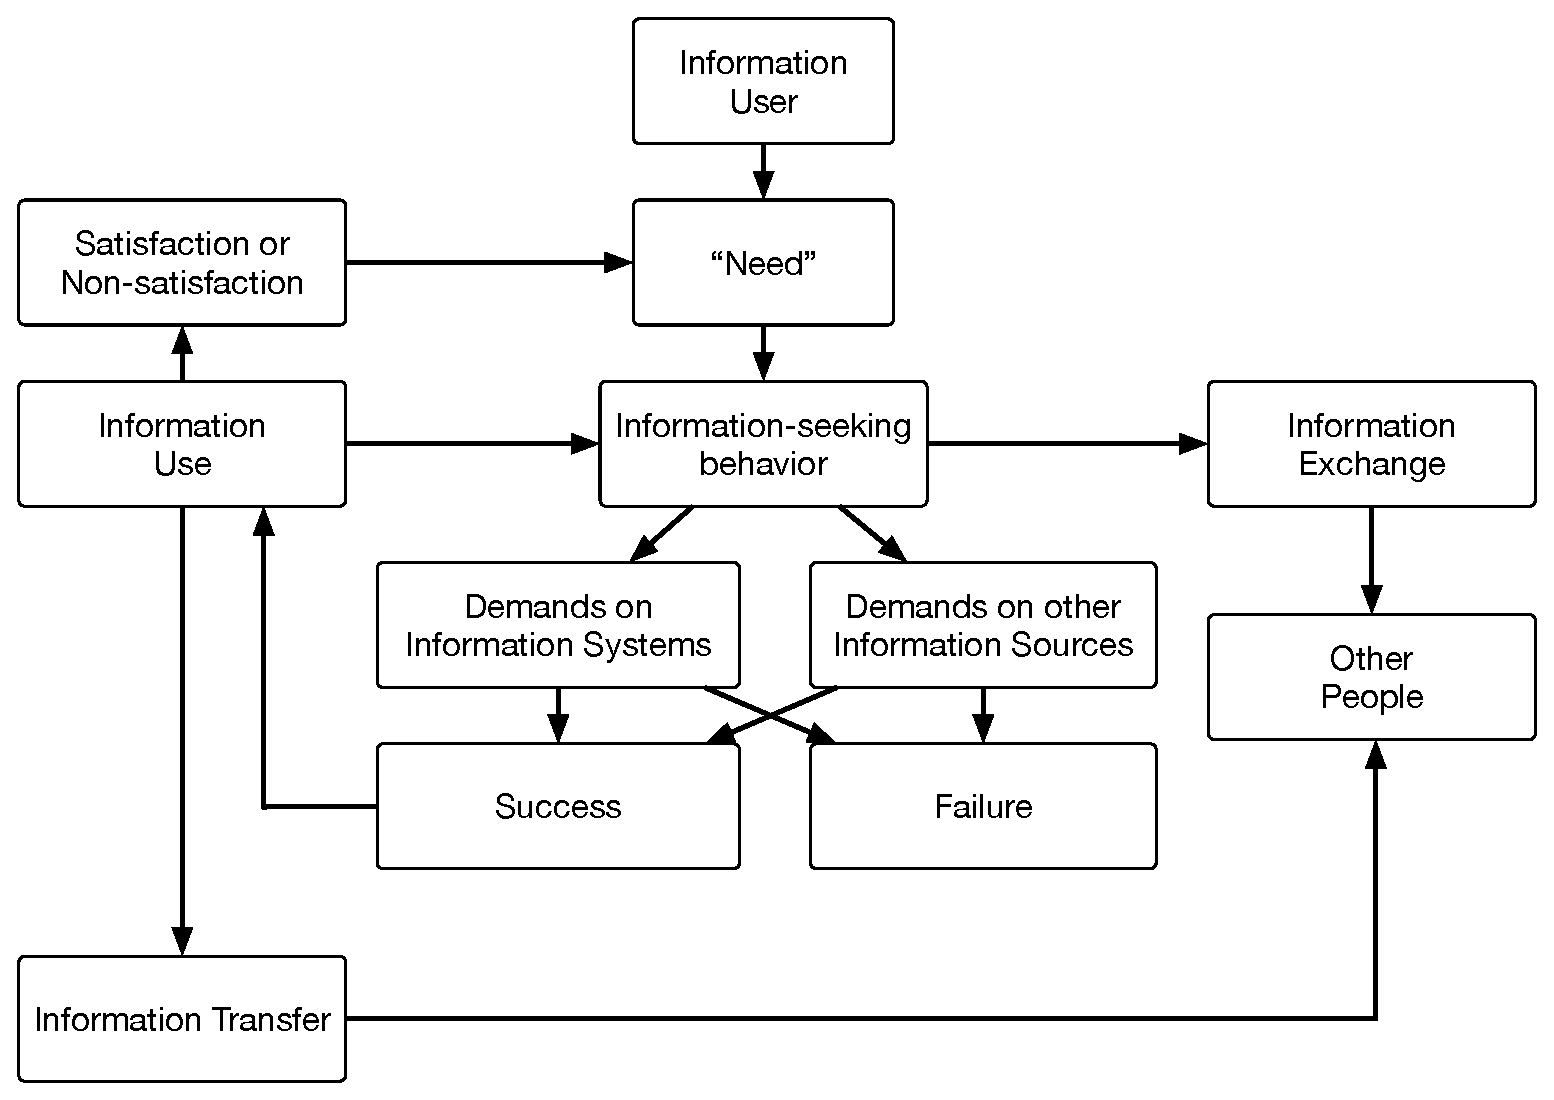
\includegraphics[width=0.7\textwidth]{figures/wilson-info-behavior}
    \caption{Wilson's information seeking behavior model \cite{wilson1981user}}
    \label{fig:wilson-info-seek}
\end{figure}

Wilson's model has been envolved many years since its origin, and it was revised 
and adapted to our digital world since the digital systems learns user preferences and 
changes \cite{giannini1998receiving} the way we receiving information.

David Ellis described a detailed group of activities for information seeking behavior \cite{ellis1989behavioural},
and then applied in physical and social science \cite{ellis1993comparison} and industrial
environment \cite{ellis1997modelling}.
In addition, his analysis was
based on grounded theory approach \cite{aceto1994grounded} and semi-structured interviews. 

Afterwards, Choo et al. adapts Ellis' Model and discussed \cite{choo1999information}
the information seeking behavior on the web through different activities rather 
than a single process, the applied activities are:
starting, chaining, browsing, differentiating, monitoring, and extracting.

``\emph{Starting}'' on the web indicates that a user identifies websites or pages
that containing the information of interests.
``\emph{Chaining}'' indicates that a user follows on starting page to other related pages.
``\emph{Browsing}'' then represents the activity that a user only skimming on the web
and quickly viewing the top-level informations. The ``\emph{differentiating}'' 
describes that a user on the web is selecting useful pages and choosing differentiated.
``\emph{Monitoring}'' activity is used for receiving updates on the sites, or revisit
the previously visited pages. Finally ``\emph{extracting}'' is the activity that a user
systematically extracts informations from a interested page or website.

By applying these activities, Choo et al concludes general user behaviors on the web are
undirected viewing, conditioned viewing, informal search and formal search.
Johnson further describes \cite{johnson2017patterns} seven more detailed behaviors 
patterns on the web, but did not given a working study that verify or prove their formation.

Although Wilson's model and Ellis' model are revised in recent works, however these improvements
are more generic and too complexy for describing user information behavior on the web.
Therefore, in this thesis, we only uses the an antecessor of Wilson's framework \cite{wilson1997information} and 
Ellis' model \cite{ellis1997modelling} to formalize and justify our lab study experiment later in Chapter \ref{ch:exp}, 
as a fundation of our work.

% \subsection{Theory of Sequence to Sequence Learning}

\cleardoublepage
\section{Action Path Models}
\label{ch:model}

\epigraph{It is impossible to separate a cube into two cubes, or a fourth power into 
two fourth powers, or in general, any power higher than the second, into two like powers. 
I have discovered a truly marvelous proof of this, which this margin is too narrow 
to contain.}{Pierre de Fermat}

In this chapter, we formalize few concepts and metrics in clickstream data,
and then describe a proposed clickstream model named \emph{Action Path model} 
based on a recurrent neural network that models a client-side web browsing behavior. 
An \emph{action path} is different than the original clickstream concept since 
a user may \emph{switch browser tabs} for parallel viewing \cite{huang2010parallel} 
or uses \emph{back button} 
for backtracking viewing \cite{huang2012no} as we discussed in Chapter \ref{ch:relate}, 
namely, a user performes a visit action.
A server-side collected clickstream does not contain such detailed level of user clickstream.
The term \emph{action path} is a generalized concept of clickstream, 
which replaces individual URLs to chronological ordered user actions 
(with back button and browser tab switch effects) in a browser.
Figure \ref{fig:clickstream} illustrates a simplified version of an action path 
that compares vanilla clickstream.

\begin{figure}[H]
    \centering
    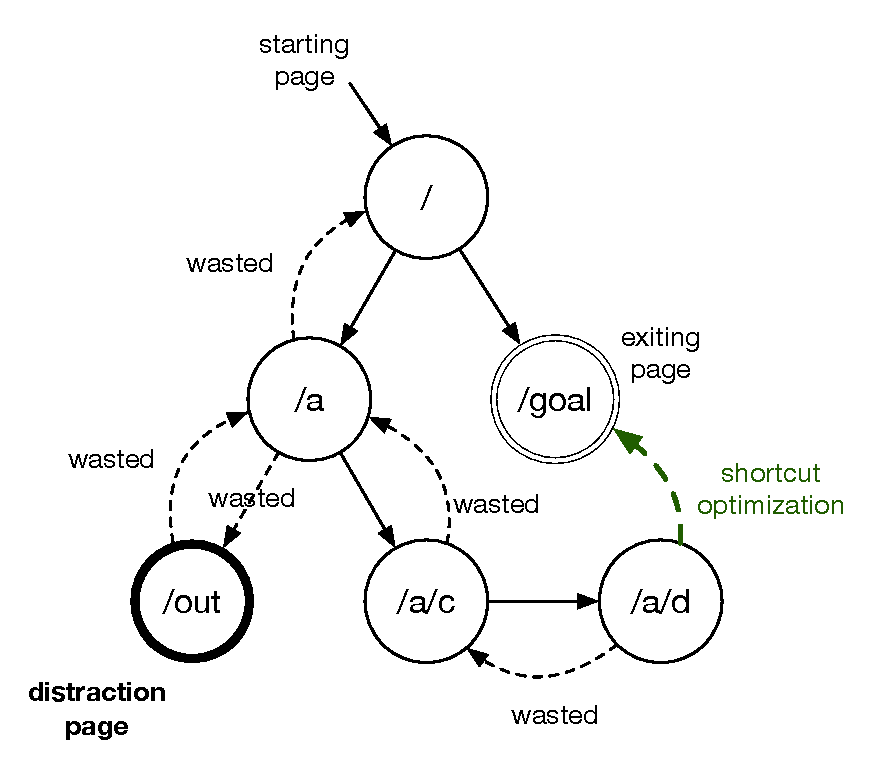
\includegraphics[width=0.5\textwidth]{figures/clickstream}
    \caption{A simple action path. A user starts from the starting page, and performed
    a series of page click actions, ends on a exiting page. 
    The server side records clickstream in the following order:
    / $\rightarrow$ /a $\rightarrow$ /out $\rightarrow$ /a/c $\rightarrow$ /a/d $\rightarrow$ /goal.
    However the actual user actions are: 
    / $\rightarrow$ /a $\rightarrow$ /out $\rightarrow$ /a $\rightarrow$ /a/c $\rightarrow$ /a/d 
    $\rightarrow$ /a/c $\rightarrow$ /a $\rightarrow$ / $\rightarrow$ /goal. 
    The records from server side lost the interaction details between users and browsers.
    Node that /out is a distraction page in the graph, 
    which may located in a different website (e.g. advertisement), 
    and black dashed arrorws are wasted user
    actions. The /goal page may not clear in the beginning of the clickstream, one can generate
    a shortcut optimization navigation to the /goal page while more clickstream context
    be presented, i.e. an optimized user action is 
    / $\rightarrow$ /a $\rightarrow$ /a/c $\rightarrow$ /a/d $\rightarrow$ /goal. In this case,
    the demand page of the visit session is discovered in /a/d.}
    \label{fig:clickstream}
\end{figure}

For the convenience of discussion, \textbf{we indiscriminate the use of 
term \emph{action path} and \emph{clickstream} in
this thesis to indicate a chronologically ordered user actions}.

\subsection{Completion Effeciency}

An action path of a visiting session starts from a starting page and ends on an existing page.
Since we consider the effect of browser back button and browser tab switches, 
a previous page could easily be visited twice, if a user clicked the back button. 
Therefore, a page may direct to multiple pages. \emph{For instance, 
an action path can degrade to a linked list if the user clicks through different pages 
without using the back button and switching tabs; or an action path can become 
a 1-to-n bipartite graph if a user use back button back to the previous page after 
clicking a page or only switching tabs from a specific page to one another}, 
as shown in Figure \ref{fig:sim-action-path}.

As a result, we define a term \emph{completion effeciency} based on shortest path from 
starting page to exiting page, and stay duration of the action path. 

\begin{figure}[H]
    \centering

\begin{subfigure}[b]{0.55\textwidth}
    \includegraphics[width=1\textwidth]{figures/linked-list}
    \caption{}
    \label{fig:sim-action-1}
\end{subfigure}
    
\begin{subfigure}[b]{0.23\textwidth}
    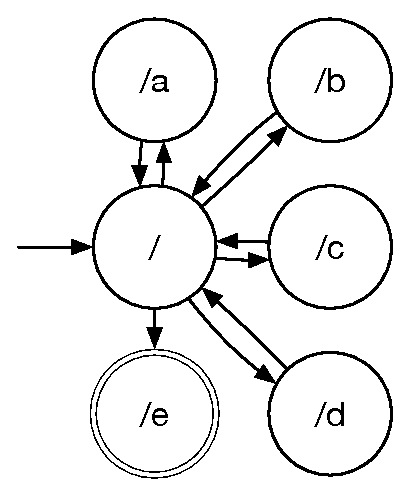
\includegraphics[width=1\textwidth]{figures/1ton}
    \caption{}
    \label{fig:sim-action-2}
\end{subfigure}

\caption{Two particular case of an action path: an action path that degrade to 
a linked list if the user click through different pages without using back button and 
switching tabs (\ref{fig:sim-action-1}), and an action path that represented 
in 1-to-n bipartite graph if a user use back button back to the previous page after 
clicking a page or only switching tabs from a specific page to one another (\ref{fig:sim-action-2}).}
\label{fig:sim-action-path}
\end{figure}

Let a directed cyclic graph represents an action path, each node represents a visited page, 
and each edge has a weight that represents the study duration of its tail node.
Assume the total stay duration of the shortest path from the starting page to 
the existing page is $d_s$, and the total stay duration of the action path is $D$, 
the number of nodes in the shortest path is $n_s$, the total nodes in an action path is $N$, 
we define the \emph{completion efficiency $E$} is as follows Equation \ref{eqn:completion-effeciency}:

\begin{align}
\label{eqn:completion-effeciency}
\begin{split}
    E = w_1 \frac{n_s}{N} + w_2 \frac{d_s}{D}\\
    w_1 + w_2 = 1
\end{split}
\end{align}

where $w_1$, $w_2$ are hyperparameters to balancing the importance of action path and 
stay duration. According to the discussion of two special cases of action path, 
it is trivial to show the range of $E$ is $(0, 1]$. As a compliment, we define 
\emph{zero completion efficiency} if and only if a user cannot complete a clickstream 
in a browsing session. Therefore we have a range of $E$ is $[0, 1]$.

\paragraph{Remark 1} The definition of completion efficiently uses the term of shortest path,
which is the problem of finding a path between the starting page and exiting page 
in an action path (directed cyclic graph) such that the sum of the stay duration of 
its constituent pages in minimized.
The problem can be solved by Dijkstra's \cite{dijkstra1959note} shortest-path algorithm. 
It selects the unvisited nodes with the smallest weights, calculates the distance 
through it to each unvisited neighbor, then updates the distance of neighbor distance 
if the distance is smaller than one another. The process converges to the shortest path.

\paragraph{Remark 2} An action path may increases with more nodes (web pages) over time.
The starting page of an active path was always the first page when the browser was opened.
However, one can always treat the currently visited page is the exiting page due to we
do not know when a user will exit browsing overtime at the moment. 
Consequently, function $E$ is changing over browsing.

\paragraph{Remark 3} We use completion efficiency as a feature for a classification task 
in Section \ref{sec:inter-general-feature}.

\subsection{\emph{url2vec} Embedding}

As we discussed in Section \ref{sec:seq-learn}, we convey similar idea from word2vec model 
and propose our \emph{url2vec} model for client side clickstream data.

The purpose of url2vec model is to construct URL representations that better predict 
the surrounding URLs in a clickstream. Briefly, given a clickstream of urls 
$\text{URL}_1, \text{URL}_2, ..., \text{URL}_T$, the objective of url2vec is to maximize 
the average log softmax probability:

\begin{align}
\label{eqn:url2vecprob}
\begin{split}
    \frac{1}{T}\sum^{T}_{t=1}\sum_{-c \leq i \leq c, i \neq 0} {\log{p(\text{URL}_{t+i} | \text{URL}_t)}}\\
    p(\text{URL}_{t+i} | \text{URL}_t) = \frac{
        \exp{(v_{\text{URL}_{t+i}} ^\top v_{\text{URL}_t})}
    }{
        \sum_{\text{all URLs}} {\exp{(v_{\text{URL}_{t+i}} ^\top v_{\text{URL}_t})}}
    }
\end{split}
\end{align}

where $c$ is the size of embedding context, which is a function of starting page,
$v_{\text{URL}_t}$ is one-hot encoded representation of input URLs, and 
$v_{\text{URL}_{t+i}}$ is the vector embedding of output representations.

\paragraph{Remark 1} The model described by Equation \ref{eqn:url2vecprob} is essentially
a three layer neural network: input layer of \emph{one-hot} encoded URLs (a group of binaries
that a component of a one-hot encoded vector is a representative of a URL under a finite set
of existing URLs), a hidden layer of feature representation and an output layer 
share weights to the learned embeddings of input URLs.

\paragraph{Remark 2} The probability in Equation \ref{eqn:url2vecprob} is impractical due to
$\nabla \log{p(\text{URL}_{t+i} | \text{URL}_t)}$ is large because of exponential terms in softmax,
two numerical optimizations \cite{mikolv2013embedding} based on Hofmann Tree and Negative Sampling
are proposed by Mikolv.

\paragraph{Remark 3} The probability can also be interpreted from a Bayesian perspective,
which provides an intuition of this definition. $p(\text{URL}_{t+i} | \text{URL}_t)$
can be considered as a posterior probability. Since $v_{\text{URL}_t}$ was initialized
as a one-hot encoded vector input to the embedding neural network, the item can be treated
as a prior, and the denominator is a normalization term.
Furthermore, the dot product between $v_{\text{URL}_{t+i}} ^\top$
and $v_{\text{URL}_t}$ is a representation of consine similarity, which represents
the closest surrounding URLs in same direction of vectors.

\subsection{Action Path Model}

Our model convey a similar idea from Stutskever's sequence 
to sequence translation as we discussed in Section \ref{sec:seq-learn}.

An \emph{action path} from user $i$ in session $j$ consist of 
a sequence of \emph{url2vec} embedded vectors $(U^{ij}_1, U^{ij}_2, ..., U^{ij}_n)$ 
and a sequence of time duration $(d^{ij}_1, d^{ij}_2, ..., d^{ij}_n)$, since each URL 
has a corresponding number that represents the time duration of a user spent on a given page.
Our action path model consist a context encoder and a context decoder that illustrated in the subsequent
subsections.

\subsubsection{Context Encoder}

\emph{Context encoder} encodes URLs one by one over timestamp and produces a context tensor 
that encodes the historical user actions, as shown in Figure \ref{fig:encoder}. 

In the encoder, we practically insert a starting mark (a mark is a special URL vector that 
differ from any other realistic URL one-hot encoded vectors) ``<SOA>'' (\emph{Start of Action})
as a sign of start feeding URLs to the encoder, and a trigger mark ``<COI>'' (\emph{Change of Intention}) as
a sign to trigger decoder to decodes encoded context tensor.

\begin{figure}
    \centering
    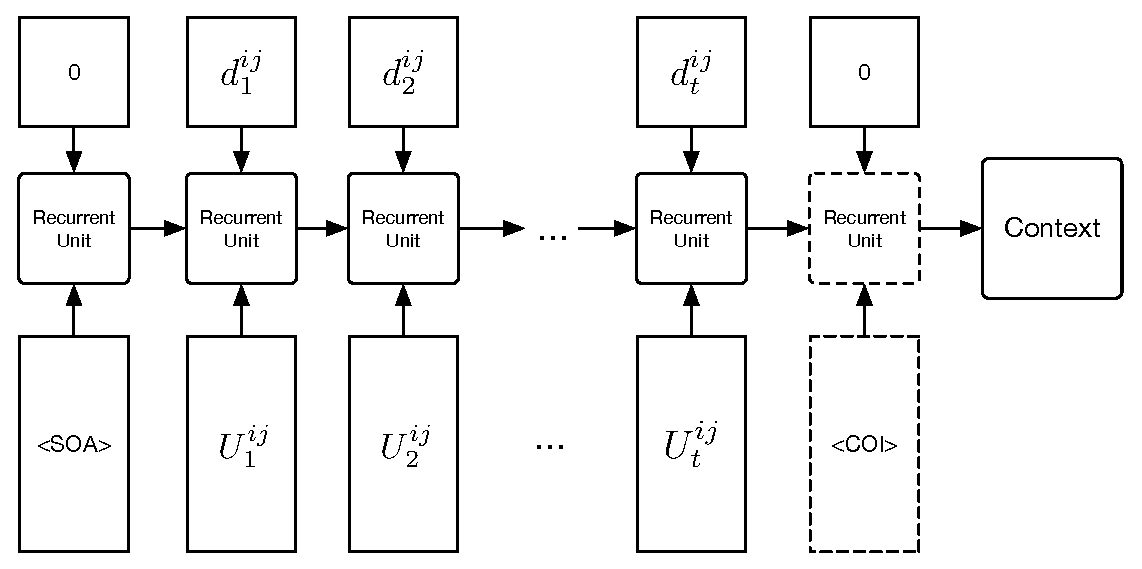
\includegraphics[width=0.7\textwidth]{figures/encoder}
    \caption{An unrolled illustration of context encoder of Action Path Model. 
    In the encoder, a starting mark ``<SOA>'' is used as a sign of start feeding URLs, 
    and a trigger mark ``<COI>'' as a sign to trigger decoder to decodes 
    encoded context tensor. The trigger mark is automatically inserted after the $k$-th URL 
    while training at the end of the encoder model over time, $k$ is increasing over time. 
    Besides, the recurrent unit is not detailly described in the figure but afterward.}
    \label{fig:encoder}
\end{figure}

Note that the input URLs to encoder's recurrent unit are preprocessed through 
url2vec embeddings, which has learned and updated from one-hot encoded vectors to 
densely distributed vectors.

\subsubsection{Context Decoder}

\emph{Context decoder} decodes the context tensor produced by the encoder into a series of URLs. 
We practically feed a prediction mark ``<SOP>'' (\emph{Start of Prediction}) 
as a sign to initiate the decoding of encoded context. 
At the end of decoder, decoder produces an ending mark ``<EOA>'' (\emph{End of Action}) 
that terminates the decoding process.

Note that the decoder model in the training phase and prediction phase is different.
In the training phase, teacher forcing strategy \cite{williams1989learning} is used, 
the strategy supplies observed user actions as inputs in the decoder.
In the evaluation phase, the decoder uses the output from the recurrent unit as an input, 
shown through dashed lines in Figure \ref{fig:decoder}.

\begin{figure}
    \centering
    \includegraphics[width=0.7\textwidth]{figures/decoder}
    \caption{The context decoder of the Action Path Model. In the decoder, 
    a prediction mark ``<SOP>'' is used to initiate the decoding process, 
    and an ending mark ``<EOA>'' as a sign to terminate decode process. 
    The output of the decoder uses a softmax intermediate operation to magnify 
    and normalize the probability of predicted URL embedding. Also, the recurrent unit 
    is not detailly described in the figure but afterward.}
    \label{fig:decoder}
\end{figure}

In our model, a decoder outputs vectors first, and we have two strategies 
in translating vectors to URLs. 
The first strategy is to use an argmax function to select the component 
with maximum probability of a vector; we use this strategy for performance evaluation 
in Section \ref{sec:eval-optimal}. Another strategy is to select a series of URLs 
that gains the highest joint probability,  we discuss and use this strategy 
for action path optimization in Section \ref{sec:optimization}.

\subsubsection{Recurrent Unit}
\label{sec:recurrent-unit}

\textbf{The recurrent unit in the Action Path model is not as standard as original 
LSTM or GRU}, which is one of the major contributions of the thesis. 
In our recurrent unit, when using LSTM as recurrent unit base, we also 
feed time duration $(d^{ij}_1, d^{ij}_2, ..., d^{ij}_n)$
into input gate $I_t$, and others (forget gate $F_t$, output gate $O_t$, 
memory cell $C_t$ and hidden state $h_t$) remains the same:

\begin{align}
\label{eqn:lstm}
\begin{split}
    I_t =& \sigma ( P^{(I)} U^{ij}_t + Q^{(I)} h_{t-1} + \frac{d^{ij}_t}{d^{ij}_t + 1}) ) \\
    F_t =& \sigma ( P^{(F)} U^{ij}_t + Q^{(F)} h_{t-1} + b^{(F)}) \\
    O_t =& \sigma ( P^{(O)} U^{ij}_t + Q^{(O)} h_{t-1} ) \\
    C_t =& F^{(t)} \circ C_{t-1} + I_t \circ \tanh (P^{(C)} U^{ij}_t + Q^{(C)} h_{t-1}) \\
    h_t =& O_t \circ \tanh (C_t)
\end{split}
\end{align}

where $t = 1, 2, ..., n; P^{(I)}, Q^{(I)}, P^{(F)}, Q^{(F)}, P^{(O)}, Q^{(O)}$ are shared weight parameters, 
$b^{(F)}$ is a bias in forget gate $F_t$,
$\circ$ represents element-wise product of two matrices.

When using GRU as recurrent unit base, we feed time duration $(d^{ij}_1, d^{ij}_2, ..., d^{ij}_n)$
in to update gate $Z_t$, and others (reset gate $R_t$, hidden state $h_t$) stay the same:

\begin{align}
\label{eqn:gru}
\begin{split}
    Z_t =& \sigma ( P^{(Z)} U^{ij}_t + Q^{(Z)} h_{t-1} + \frac{d^{ij}_t}{d^{ij}_t + 1} ) \\
    R_t =& \sigma ( P^{(R)} U^{ij}_t + Q^{(R)} h_{t-1} ) \\
    h_t =& ( 1 - Z_t ) \circ \tanh ( P^{(H)} U^{ij}_t + Q^{(H)} h_{t-1} ) + Z_t \circ h_{t-1}
\end{split}
\end{align}

where $t = 1, 2, ..., n; P^{(Z)}, Q^{(Z)}, P^{(R)}, Q^{(R)}, P^{(H)}, Q^{(H)}$ are shared weight parameters, 
$\circ$ represents element-wise product of two matrices.

\paragraph{Remark 1} The units we described in this section is neither LSTM nor GRU since
the input gate $I_t$ or update gate $Z_t$ introduces time duration $d^{ij}_t$ as input,
which is different from a simple constant bias in the first learnable bias in these gates. 
It is worth mentioning that adding bias to the gates are helpful to 
improve learning performance in LSTM \cite{Jozefowicz:2015:EER:3045118.3045367}, 
we also use the trick in our model as shown in $F_t$ of Equation \ref{eqn:lstm}.

\paragraph{Remark 2} The term $\frac{d^{ij}_t}{d^{ij}_t + 1}$ is a squashing mechanism,
it normalizes $d^{ij}_t$ from $(0, \infty)$ to $(0, 1)$.

\subsubsection{Ending Mark Interpretation}
\label{sec:mark-interpretation}

In context decoder, we mentioned an ending mark ``<EOA>'' that indicates the 
termination decoding process. However, the ending mark is different from other marks, 
since in practice, ``<EOA>'' is represented in different symbols of 
behavior-based categorical clickstream, which as a label to 
involve classification of user actions.

Assume action paths are labeled by one-hot encoded ending marks 
$\text{EOA}_1, \text{EOA}_2, ..., \text{EOA}_m$ and the last output
of decoder hidden state is $h_n$, we have:

\begin{align}
\label{eqn:mark}
\begin{split}
    \hat{y} =& \text{argmax} (\text{softmax} (W^{(M)} h_n)) \\
    \hat{y} \in& \{ \text{EOA}_1, \text{EOA}_2, ..., \text{EOA}_m \}
\end{split}
\end{align}

where $W^{(M)}$ is a weight parameter, and $m$ is the number of ending mark categories.

\subsection{Action Path Optimization}
\label{sec:optimization}

In traditional classification models, the arguments of the maxima (argmax) are used 
to select labels with the highest probability, scilicet, argmax selects predicted URLs 
with the highest probability of user action from decoder outputs. However, this method 
is under the condition of all outputs are independent in probability, which 
is not suitable for our action path optimization scenario.

In previous sections, our model feeds an input clickstream $(U^{ij}_1, U^{ij}_2, ..., U^{ij}_t)$,
and produce an output $(o_1, o_2, ..., o_{m})$ that expect close to actual clickstream 
$(U^{ij}_{t+1}, U^{ij}_{t+2}, ..., U^{ij}_n)$.
Then the probability of expected clickstream is a conditional probability under 
the input clickstream. In other words, we need to solve an optimization problem:

\begin{align}
\label{eqn:optimize}
\begin{split}
    & \operatorname*{argmax}_{o} p( o_1, o_2, ..., o_{m} | U^{ij}_1, U^{ij}_2, ..., U^{ij}_t ) \\
   =& \operatorname*{argmax}_{o} \prod_{k=1}^{m} p(o_{k} | U^{ij}_1, ..., U^{ij}_t, o_1, ..., o_{k-1}) \\
   =& \operatorname*{argmax}_{o} \sum_{k=1}^{m} \log p(o_{k} | U^{ij}_1, ..., U^{ij}_t, o_1, ..., o_{k-1})
\end{split}
\end{align}

A heuristic approach can solve the optimization problem efficiently, namely beam search 
\cite{DBLP:journals/corr/abs-1211-3711}.
In each step of decoder output, we reserve the top-$k$ best combinations of URLs and 
eliminate the rest of URLs from evaluation, and finally selects $k$ best clickstreams.
The pseudocode is given that adapts vanilla beam search to URL prediction search 
in Algorithm \ref{algo:optimize}.

~\\

\begin{algorithm}[H]
\label{algo:optimize}
\SetAlgoLined
\SetKwInOut{Input}{input}\SetKwInOut{Output}{output}
\Input{Decoder outputs $(o_1, o_2, ..., o_{m})$,\\
        Number of candidates $k$}
\Output{k clickstream candidates with highest probability}
\Begin{
    Initialize empty $\text{clickstreams}$ list \\
    \For{$o$ $\in$ $(o_1, o_2, ..., o_{m})$}{
        Initialize empty $candidates$ list \\
        \For{$\text{clickstream}$ $\in$ $\text{clickstreams}$}{
            \For{page $\in$ $o$)}{
                candidates.append([clickstream.append(page), $log(p(\text{clickstream})) + log(p(\text{page}))$]) \\
            }
        }
        ordered = descending order sort candidates by score \\
        clickstreams = ordered[:k]
    }
}
\caption{Output Clickstream Search}
\end{algorithm}

~\\

\paragraph{Remark} The algorithm produces a heuristic output with given clickstream context. 
Combining with the \emph{url2vec} model, the prediction
can heuristically optimize the click path of a specific user since the embeddings 
are trained over all possible action path. For instance, 
a distraction advertisement page will not appear
after optimization because the embedding of the advertisement page 
is far from the desired page if embeddings are learned correctly.

\cleardoublepage
\section{Experiment}
\label{ch:exp}

In this chapter, we rationalize the process of our lab study based on the theory of
human information behavior, then construe 
the purpose of context given web browsing tasks to our subjects.

The lab study took place during the last two weeks of November, from 14/11/2018 to 29/11/2018
in Frauenlobstrasse 7a, a faculty building of Ludwig-Maximillians-Universitaet Muenchen.
Client-side user clickstream data was collected by a embedded collector plugin installed in 
the mainstream browser, i.e. Google Chrome, on a self provided desktop computer and a laptop.

In lab study, we select three mainstream websites, Amazon/Medium/Dribbble, 
that covers categories for shopping, media consuming and design brainstorming with design 
reasons (discuss later in Section \ref{sec:task-design}).
Then we manually designed 35 reasonable tasks and finally selected 9 
context-given browsing tasks (three for each website, discuss in 
Section \ref{sec:task-design}) to simulate three different proposed browsing behavior,
namely goal-oriented/fuzzy/exploring behaviors.
Each task requires participant start from a starting page of a given website, and
all tasks do not restrict participants use the given website, but also allow they 
access websites outside the landing page to help they complete the task (explicitly informed to 
participants before participation).
Participants start browsing after they completely understand the requirements of 
each task, and no interruption or question answering during the task
except exceeding time limit of a task, however subjects can either acquire more time 
to accomplish the task or give up directly.

The study is designed as a within-subject study, thus every participant performs all tasks. 
To eliminate the learning effect due to the long time of using same websites, 
we use Latin square \cite{cochran1950experimental} 
for the device (Desktop/Laptop) and tasks participation order to our participants.

Our lab study obtained 21 participants with a mean age of 23.04 (standard deviation of 3.216, min=18 and max=19) 
took part in the study, 10 male and 11 female, whom are recruit anonymously and 
randomly via a mailing list.

\subsection{Environment}

The lab study uses two self provided devices: a desktop computer and a mobile laptop.
The reason of choose two morphology of computing device is our study requires recording
a complete clickstream of during the study.

A major issue of mobile devices is the operating system installed in mobile phone does not
authorize the permission of allowance to collect data precisely over pages or user actions.
Though Android device can overpass system permission to privilge, the user behavior 
between iOS and Android device is still completely different with different models (TODO: cite support). 
Subjects shows abnormal behavior when they use a newly provided device. 
Therefore we stick our study environment to desktop devices, 
which empower us easily collects the clickstream data from browsers with plugin supports.

Although all modern browsers support plugin development, considering the usage share of 
all browsers on the market, Google Chrome \cite{wiki2018share} obtains 61.7\% 
market shares of desktop browsers, and Apple Safari only shares
15.0\% of the market. Clearly, Google Chrome dominant market of the desktop web browser.

Hence, we decide to use Chrome to establish our plugin of data collection.
The quesionaire after our lab study indicates the browsers usage share of all subjects, 
as shown in Table \ref{table:sharesubjects}, which further supports our decision of 
browser selection.

\begin{table}[H]
    \small
    \centering
    \setlength{\belowcaptionskip}{10pt}
    \caption{Browser Usage Shares of Lab Study Subjects}
    \begin{tabular}{ccccc}
          \toprule
        & \textbf{Google Chrome} & \textbf{Apple Safari} & \textbf{Mozilla Firefox} & \textbf{Microsoft Edge} \\
          \hline
          Number     & 11 & 5 & 3 & 2 \\
          Percentage & 52.38\% & 23.81\% & 14.29\% & 9.52\% \\
          \bottomrule
    \end{tabular}
    \label{table:sharesubjects}
\end{table}

% \subsection{Context-given Websites}

% In our study, we gathered various websites covering most of the categories that people do
% on the Internet: Social Networks, Shopping, Email, Media Consuming, Search, Production 
% and etc \cite{lori2018internet, lori2017internet}. All selected website are listed 
% in Table \ref{table:websites}.

% \begin{enumerate}
%     \item social network: facebook / twitter / weibo
%     \item shopping: amazon.com / ebay.com
%     \item search: google.com / bing.com / baidu.com
%     \item media: medium.com
%     \item development: github.com
%     \item design dribbble.com
%     \item study medien.ifi.lmu.de
%     \item study en.uni-muenchen.de
%     \item streaming media youtube.com
%     \item research arxiv.com
%     \item study ielts.org
%     \item media bloomberg.com/europe
%     \item social community reddit.com
% \end{enumerate}

% \begin{table}[H]
%     \small
%     \centering
%     \setlength{\belowcaptionskip}{10pt}
%     \caption{Browser Usage Shares of Lab Study Subjects}
%     \begin{tabular}{ccccc}
%           \toprule
%         & \textbf{Google Chrome} & \textbf{Apple Safari} & \textbf{Mozilla Firefox} & \textbf{Microsoft Edge} \\
%           \hline
%           Number     & 11 & 5 & 3 & 2 \\
%           Percentage & 52.38\% & 23.81\% & 14.29\% & 9.52\% \\
%           \bottomrule
%     \end{tabular}
%     \label{table:sharesubjects}
% \end{table}

% \subsection{Pilot Study}

% Initially, we developed a web crawler that downloaded the entire medien computer science website 
% \footnote{\url{https://medien.ifi.lmu.de}}
% .... TODO discuss how we go here?


\subsection{Browsing Behaviors}
\label{sec:behavior}

Before we explain the foundation theory and design reason of our context-given browsing task, 
we first present and discusses three common types of user browsing behavior: \textbf{goal-oriented}, 
\textbf{exploring} and \textbf{fuzzy}.

These three terminologies are aggregated and incorporated from behaviors that concluded in former 
qualitative researches, all these terminologies are based on a fundmental theory of 
interdisciplinary perspective information seeking behavior and human information behavior\cite{wilson1997information} 
as we discussed in Section \ref{sec:info-seek}. TODO:
Table \ref{table:info-seek} compares the differences between former research and ours.

\begin{table}[H]
    \small
    \centering
    % \setlength{\belowcaptionskip}{10pt}
    \caption{Terminologies comparison of information behavior on the web}
    \begin{adjustbox}{width=\textwidth}
        \begin{tabular}{ccccc}
            \toprule
            \textbf{Author} & \textbf{Terminologies} & \textbf{Terminologies} & \textbf{Terminologies} & \textbf{Main Factors} \\
            \hline
            \cite{choo1999information} & Formal search & \makecell{Conditioned viewing; \\ Informal search} & Undirected viewing & \makecell{Psychological; demographic;\\ role-related environmental; \\source characteristics} \\
            \cite{johnson2017patterns} & \makecell{Directed browsing; \\Known-item search} & \makecell{Semi-directed browsing; \\Explorative seeking; \\``You do not know what you need''; \\Re-finding} & Undirected Browsing & Behavior \\
            \textbf{This thesis} & \textbf{Goal-oriented} & \textbf{Fuzzy} & \textbf{Exploring} & \textbf{Purpose} \\
            \bottomrule
        \end{tabular}
        \label{table:info-seek}
    \end{adjustbox}
\end{table}

As justification, we combines Ellis' Model and ``information use'' behavior proposed in
information behavior theory to justify our summarized behaviors:

\paragraph{Goal-oriented behavior} occurs when a user initiate 
visiting session on the web caused by a determined objective in a specific context, 
such as bussiness work, 
social communication, university study, literature research and etc. 

Goal-oriented behavior indicates an actively information seeking behavior.
Instead of \emph{formal search}, that only covers the phase of ``monitoring'' and ``extracting''
(or \emph{directed browsing} and \emph{known-item search} that covers ``browsing'' and ``differentiating'' or 
``monitoring'' and ``extracting'' respectively), 
goal-oriented browsing behavior contains the entire life cycle of human information behavior starts
from ``starting''. Under browsing behavior, a determined ``information use'' can be observed
or concluded.

For instance, a college student intentionally need a latest lecture slide (\emph{information use} observed), 
the student then opens web browser, access college website (\emph{starting}) and navigates to the lecture homepage 
(\emph{chaining}, \emph{browsing}, and \emph{differentiating}).
Finally, the student exit browsing after download the slides (\emph{monitoring} and \emph{extracting}).

\paragraph{Exploring behavior} occurs when a user initiates browsing session aimlessly with no clear observed
extracting or information use during the session, the person greedily or breadth-first consumes and the content on the Web without 
any information extracting and information use, such as media consuming, learning before using and etc.

Exploring browsing behavior indicates a complete opposite behavior comparing to 
goal-oriented borwsing behavior. More formally describing exploring behavior using Ellis' model, 
the behavior represents ``chaining'' and ``browsing''
without ``differentiating'' and ``extracting'' from ``starting'' while information seeking.

For instance, a person who accesses an unknown utility web application (\emph{starting}), he/she explores
what functions are provided one by one and what he/she can do while using the application
(\emph{chaining} and \emph{browsing}).

\paragraph{Fuzzy behavior} occurs when a user initiate visiting session for information use
 with non-systematic, incomplete prior knowledge that may browsing ongoing for updating 
the framework of knowledge until final acquisition or abandon.

Fuzzy behavior in a browsing behavior in between of goal-oriented and exploring behaviors.
Instead of only ``chaining'' and ``browsing'' from ``starting'', fuzzy behavior also do
``differentiating'' or ``monitoring'' while information seeking.

For instance, a researcher heared a new technique proposed in another scientific field 
that may influence he/she's research, then the person 
opens a search engine (\emph{starting} and \emph{chaining}) to seek (\emph{browsing}) existing (\emph{differentiating}) 
follow up researches (\emph{monitoring}). The browsing may ends without information use
because of the technique is irrelevant to he/she's research.

\paragraph{Remark} Table \ref{table:ellis} illustrates a mapping from these three
browsing behavior to the complete human information behavior.
Note that ``information needs'' is not suggested in T. Wilson's theory since
``information needs'' is not 

\begin{table}[H]
    \small
    \centering
    % \setlength{\belowcaptionskip}{10pt}
    \caption{Terminologies comparison of information behavior on the web}
    \begin{adjustbox}{width=\textwidth}
        \begin{tabular}{ccccc}
            \toprule
            \textbf{Author} & \textbf{Terminologies} & \textbf{Terminologies} & \textbf{Terminologies} & \textbf{Main Factors} \\
            \hline
            \cite{choo1999information} & Formal search & \makecell{Conditioned viewing; \\ Informal search} & Undirected viewing & \makecell{Psychological; demographic;\\ role-related environmental; \\source characteristics} \\
            \cite{johnson2017patterns} & \makecell{Directed browsing; \\Known-item search} & \makecell{Semi-directed browsing; \\Explorative seeking; \\``You do not know what you need''; \\Re-finding} & Undirected Browsing & Behavior \\
            \textbf{This thesis} & \textbf{Goal-oriented} & \textbf{Fuzzy} & \textbf{Exploring} & \textbf{Purpose} \\
            \bottomrule
        \end{tabular}
        \label{table:ellis}
    \end{adjustbox}
\end{table}

\subsection{Tasks Design}
\label{sec:task-design}

We designed 35 browsing tasks, after conduct a pilot study, 
9 tasks are selected for three websites: Amazon.com, Medium.com and Dribbble.com 
because of the following reasons:

\begin{enumerate}
    \item These three websites all have coresponding tasks to the three type of browsing behavior;
    \item Each of the task can be finished around 5 to 10 minutes;
    \item All these websites are mainstream websites, they do not require 
        massive professional domain knowledge for using.
\end{enumerate}

Moreover, the unselected tasks are listed in Appendix \ref{appendix:unselected}.

\subsubsection{Goal-oriented Task}

We designed and selected an appropriate goal-oriented task for selected websites respectively,
and each task is designed with three determined goal.

\begin{itemize}
    \item \textbf{Amazon.com}: \emph{Assume your smartphone was broken and you have 1200 euros 
    as your budget. You want to buy an iPhone, a protection case, and a wireless 
    charging dock. Look for these items and add them to your cart.}

        This task contains three determined purpose since a subject is required to add three items
        to the cart. There are few hidden consideration behind the task, which makes the task
        more realistic: a) There is a budget of this task, which requires subjects must consider the
        price of items instead of simply add the first recommended item to cart; 
        b) the starting page is amazon.com instead of amazon.de. This decision requires
        subjects must also consider the currency rate between US dollars and Euros for budget.
        c) There are some items cannot be shipped to Germany (the study took place in Germany).
        As a result, subjects cannot add these items to cart and they should find other alternatives.

    \item \textbf{Medium.com}: \emph{Assume you were making plans for your summer vacation. 
        You want to visit Tokyo, Kyoto, and Osaka. You want to find out what kind of experience other people made 
        when traveling to these three places in Japan. Your task is to find three posts 
        for traveling tips regarding these cities. Elevate a post if it is one of your choices.}

        This task contains three determined purpose since there are three fixed traveling destination.
        The task also implies few considerations that increase the required interaction of the task to subjects:
        a) The website only offers English version, some Japanese character may appear in an article,
        thus, a translation util may be used while the study;
        b) An article may apears numerous noun, such as toponym. Search engine may used while the study;
        c) the articles, those require a membership to unlock reading, cannot be elevated. 


    \item \textbf{Dribbble.com}: \emph{You are hired to a Cloud Computing startup company. You get an assignment to 
        designing the logo of the company. Search for existing logos for inspiration and 
        download three candidate logos you like the most.}

        The task also has three determined prupose since subjects are quired to download three candicate trademarks.
        While the participation, subjects still need take few implicit facts in to account:
        a) Subjects who unfamiliar with the term "Cloud Computing" need visit other explainations to figure out
        the vision and mission of this type of company, and subjects whom already familiar with the term
        still need to compares the designed made by other competitors.
        b) Subjects should aware some of the designs shared on the website are not suitable for trademark or icon design.
\end{itemize}

\subsubsection{Exploring Task}

Exploring tasks simply do not provides any deterministic objective,
and all websites has a designed exploring task for subjects.

\begin{itemize}
    \item \textbf{Amazon.com}: \emph{Look for a product category that you are interested in and start browsing. 
        Add three items to your cart that you would like to buy.}

        Although the task do not require any specific items to the subjects, the task remains three different
        purpose because participants need add three items to the cart. This designed task 
        is aimlessly because: all tasks is not formerly informed to participants, 
        they either do not have needs of buying items or 
        formerly exist needs of buying a specific category but do not have a product candicate yet.
        Besides, the description of the task ask participants start from a product category, which avoids 
        goal-oriented buying a specific product.

    \item \textbf{Medium.com}: \emph{Visit a category you are interested in and elevate three post you like.}

        Similar reason as discussed in Amazon.com's exploring task. It is well to be remined that Medium is a media
        website, visiting a specific article formerly read before participation is relatively difficult 
        since all contents showed to users are daily updated. Thus the task can be directly consider as an exploring task.

    \item \textbf{Dribbble.com}: \emph{Explore dribbble and download three images you like the most while you browse.}

        Dribbble illustrates designs by using image gallery. The major difference between Dribbble and Google Image Search
        is dribbble is a user-centered content aggregation website, but Google Image Search is a simple content aggregation engine.
        As a result, there will be two different interaction in Dribbble: exploring designs based on keywords and categories,
        or exploring designs based on users. The latter can helps its user finding similar designing style.
        The task is aimlessly since the task simply describes nothing and completely let participants explore their preferences.

\end{itemize}

\subsubsection{Fuzzy Task}

Each of our selected websites also has an fuzzy task respectively, and there are three major goals per task.

\begin{itemize}
    \item \textbf{Amazon.com}: \emph{You want to buy a gift for your best friend as a birthday present.
        Add three items to your cart as candidate.}

        The clearness of the task is stronger than exploring task but weaker than goal-oriented task, because
        The task restricts participants adding items for a specific purpose (birthday present) but not points
        any specific product.

    \item \textbf{Medium.com}: \emph{Assume you got an occasion to visit China for business. 
        You are free to travel to China for a week. 
        You want to make a travel plan for touring China within a week. Your task is to find out what kind 
        of experience other how people made when going to secondary cities or towns in China, then decide 
        on three cities you want to visit (excluding  Beijing, Shanghai, Guangzhou, and Shenzhen). 
        Elevate if a post helped you make a decision.}

        The clearness of the task is stronger than exploring task, because it asks a participant 
        to exploring a non-deterministic direction of looking for secondary cities.
        But the clearness of the task is weaker than goal-oriented task due to secondary cities described
        in Medium's user posts is unclear, participants suppose to make decision themselves.
        Furthermore, this ask is asking regarding traveling China around a week. Cities cannot be randomly
        selected because to make traveling plan requires consider geographic location of the city.

    \item \textbf{Dribbble.com}: \emph{You are preparing a presentation and need one picture for each of these animals: 
    cat, dog, and ant. Download the three pictures you like the most.}

        The task has three purpose of downloading images of animals, which restrict participant to a specific direction,
        thus, the clearness of the task is stronger than exploring task. However, the task describes a scenario of using
        these images in a presentation, and hence participants must consider continuity of design style, which makes
        the clearness of the task is weaker than goal-oriented task. 
\end{itemize}

\cleardoublepage
\section{Evaluation}
\label{ch:eval}

\epigraph{If a machine is expected to be infallible, it cannot also be intelligent.}{Alan Turing}

In this chapter, we conduct evaluations to our collected data.
The data is collected from 21 subjects, and 189 clickstream data are collected in total. 
Each clickstream contains action-level data with a stay duration
of a specific page, for instance, we still collect an URL as a step of clickstream 
if a participant uses back button rollback to a previous visited page without requesting server. 
A clickstream also has a subjective difficulty score from questionaire (shown in Appendix \ref{appendix:b}) 
after the completion of each task.

\subsection{Subjective Task Difficulty}
\label{sec:task-diff}

This section discusses the subjective task difficulty qualitatively and quantitatively.
Figure \ref{fig:difficulty} illustrates a normalized (raw scores are listed in 
Appendix \ref{appendix:c} Table \ref{table:diff-raw}) subjective difficulty score 
with respect to all tasks.

\begin{figure}[H]
    \centering
    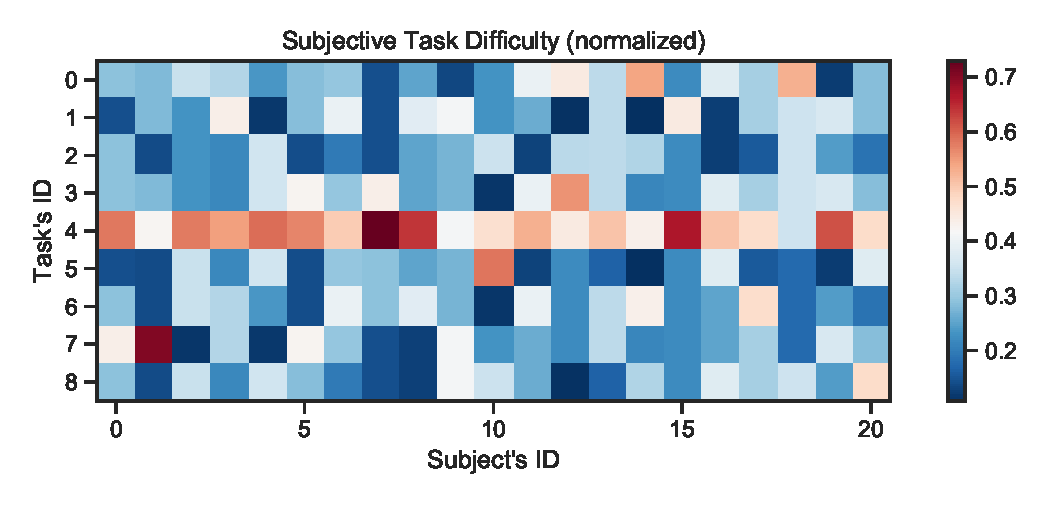
\includegraphics[width=0.7\textwidth]{figures/difficulty}
    \caption{Subjective difficulty score: each column indicates an individual subject and
    each row indicates a browsing task. Tasks from 0 to 8 represent Amazon Goal Oriented Task,
    Amazon Fuzzy Task, Amazon Exploring Task; Medium Goal Oriented Task, Medium Fuzzy Task,
    Medium Exploring Task, Dribbble Goal Oriented Task, Dribbble Fuzzy Task and Dribbble Exploring Task
    respectively.
    From this heat map, we clearly observes Medium Fuzzy Task is the most difficulty task
    according to the subjects voted subjective difficulty, a Mann-Whitney U significant 
    test justifies this observation.}
    \label{fig:difficulty}
\end{figure}

To generalize the task difficulty, the null hypothesis ($H_0$): the difficulty of fuzzy task is not greater
than exploring task and alternative hypothesis ($H_1$): the difficulty of fuzzy task is greater than
exploring task. We conduct non-parametric one-tailed Mann-Whitney U test \cite{mann1947test}, 
under null hypothesis, $p=2.54\times 10^{-5} < 0.05$, reject $H_0$.
Similarly, we compare difficulty score on goal oriented task and exploring task (with corresponding hypothesis, 
$p=0.00534 < 0.05$), difficulty score on fuzzy task and goal oriented task (with corresponding hypothesis, 
$p=0.0145 < 0.05$), all rejects $H_0$. Therefore we concludes the task difficulty is ordered
as follows: \emph{difficulty of fuzzy task $>$ difficulty of goal oriented task $>$ difficulty of exploring task},
which means exploring tasks have lower effort in clickstream, and effort of doing fuzzy task gains highest effort.

\subsection{Browsing Behavior Classification}

As discussed in Section \ref{sec:task-design}, we described three type of browsing behavior. 
In this section, we provides two type of evaluations to interpret the browsing behavior classification.

First, we evaluate the indication of general features browsing behavior,
features including difficulty of task, number of actions in a clickstream as well as the total stay duration in a clickstream.
Then we implements our action path model by using the action-level clickstream data and stay duration of each page,
which was described in Section \ref{sec:recurrent-unit} and \ref{sec:mark-interpretation}.

\subsubsection{Interpretation based on General Features}
\label{sec:inter-general-feature}

As a baseline of our classification performance, we use the \textbf{completion efficiency}, 
\textbf{total time duration of a task} 
as well as \textbf{total number of actions of a task} as the three features for
browsing behavior classification.

Note that the completion efficiency is defined by the shortest path of entire clickstream,
 and the completion efficiency cannot can only be determined if and only if the clickstream
 is given, in a sense, it carries a latent information of browsing behavior.

We applied gird-search on support vector machine (SVM) with polynomial kernel,
the best classification precision is 0.53 ($C=4.5, \gamma = 1.5$),
and the micro average F1 score is also 0.53, which is better than random (0.33).

\begin{figure}
    \centering

    \begin{subfigure}[b]{0.45\textwidth}
        \includegraphics[width=1\textwidth]{figures/tsne-amazon}
        \caption{}
        \label{fig:tsne-amazon}
    \end{subfigure}
    \begin{subfigure}[b]{0.45\textwidth}
        \includegraphics[width=1\textwidth]{figures/2d-eff-dur-amazon}
        \caption{}
        \label{fig:2d-eff-dur-amazon}
    \end{subfigure}
    \begin{subfigure}[b]{0.45\textwidth}
        \includegraphics[width=1\textwidth]{figures/2d-eff-len-amazon}
        \caption{}
        \label{fig:2d-eff-len-amazon}
    \end{subfigure}
    \begin{subfigure}[b]{0.45\textwidth}
        \includegraphics[width=1\textwidth]{figures/2d-len-dur-amazon}
        \caption{}
        \label{fig:2d-len-dur-amazon}
    \end{subfigure}

    \caption{In these figures, \ref{fig:tsne-amazon} shows the t-SNE projection
    of completion efficiency, total time duration and number of actions for three different behavior;
    \ref{fig:2d-eff-dur-amazon} is a 2D comparasion of using completion efficiency and total time duration;
    \ref{fig:2d-eff-len-amazon} provides a 2D comparasion of using completion efficiency and number of actions;
    \ref{fig:2d-len-dur-amazon} shows a 2D comparasion of using number of actions and total time duration.
    From t-SNE visualization, we observed that exploring tasks tend to centralized on the right and goal-oriented
    tasks and fuzzy tasks tend to centralized on the left, which indicates that exploring behaviors tend to classifiable
    comparing to other two behaviors. According the rest of feature comparasion visualizations, the completion effeciency and total time duration
    contributes more on interpret exploring behavior, and the number of actions tent to
    contributes more on interpret goal-oriented task.}
    \label{fig:general-amazon}
\end{figure}

To understand the meaning of classification, we also applies a randomized decision tree
that gives the importance of the used features: \emph{total time duration and number of actions
of a task is more important than our self defined completion efficiency.}

More specifically, we applies one-tailed Mann-Whitney U test for each of the features,
for instance the null hypothesis ($H_0$): the completion efficiency of goal-oriented task 
is not greater than exploring task, we have $p = 0.0019 < 0.05$ reject $H_0$, which means
the completion efficiency of goal-oriented task is significant efficient than than exploring task.

Similarly, we conduct the significant test with similar hypothesis 
to all comparable combinations as showed in Table \ref{table:sig-test-efficiency}, \ref{table:sig-test-duration}, and \ref{table:sig-test-actions}.

\begin{table}[H]
    \small
    \centering
    \caption{One-tailed significant test for completion efficiency in different browsing behaviors.
    The null hypothesis in this table, for instance, completion efficiency of fuzzy task
    is \emph{not} significant efficient than goal-oriented task, the result $p=0.45>0.05$ which means
    accept $H0$. Similar to others.}
        \begin{tabular}{cccc}
            \toprule
              v.s.             & efficiency goal & efficiency fuzzy & efficiency explore \\
            efficiency goal    & N/A             & reject           & reject             \\
            efficiency fuzzy   & accept          & N/A              & reject             \\
            efficiency explore & accept          & accept           & N/A                \\
            \bottomrule
        \end{tabular}
        \label{table:sig-test-efficiency}
\end{table}

\begin{table}[H]
    \small
    \centering
    \caption{One-tailed significant test for total stay duration of a task in different browsing behaviors.
    The null hypothesis in this table, for instance, total stay duration of fuzzy task
    is \emph{not} significant stay longer than goal-oriented task, the result $p=0.41>0.05$ which means
    accept $H0$. Similar to others.}
        \begin{tabular}{cccc}
            \toprule
              v.s.             & duration goal & duration fuzzy & duration explore \\
            duration goal      & N/A & reject & reject \\
            duration fuzzy     & accept & N/A & reject \\
            duration explore   & accept & accept & N/A \\
            \bottomrule
        \end{tabular}
        \label{table:sig-test-duration}
\end{table}

\begin{table}[H]
    \small
    \centering
    \caption{One-tailed significant test for total number of actions of a task in different browsing behaviors.
    The null hypothesis in this table, for instance, total number of actions of fuzzy task
    is \emph{not} significant performs more actions than goal-oriented task, the result $p=0.019<0.05$ which means
    reject $H0$. Similar to others.}
        \begin{tabular}{cccc}
            \toprule
              v.s.             & actions goal & actions fuzzy & actions explore \\
              actions goal      & N/A & accept & reject \\
              actions fuzzy     & reject & N/A & accept \\
              actions explore   & accept & reject & N/A \\
            \bottomrule
        \end{tabular}
        \label{table:sig-test-actions}
\end{table}

As conclusions, we summarized that:

\begin{itemize}
    \item \textbf{Completion efficiency}: the completion efficiency of goal-oriented and fuzzy behavior is significant efficient than exploring behavior;
    \item \textbf{Number of actions}: the number of actions of goal-oriented behavior is significant lower than fuzzy and exploring behaviors.
    \item \textbf{Total stay duration}: the total stay duration of explroing behavior is significant higher than goal-oriented and fuzzy behaviors.
\end{itemize}

Furthermore, the completion efficiency and total stay duration are the more important than others for indication of exploring behavior,
and number of actions are more important than others for indication of goal-oriented behavior.

\subsubsection{Intepretation based on Action Path}
\label{sec:inter-action-path}

To use full capacity of our data, this section uses the entire clickstream and its corresponding
page-level stay duration as input, three ending mark (<EOA\_GOAL>, <EOA\_FUZZY>, and <EOA\_EXPLORE>) 
as classification outputs, and then implements a single GRU layer action path model 
to classify the three type of browsing behaviors.

Our training parameters are: 
The GRU latent dimension is 10, training process feeds 132 clickstreams as training data,
38 clickstreams as validation, then 
propagates 500 epochs with batch size of 32. In the training process, we use Adam optimizer,
 categorical corss-entropy loss as well as L1 and L2 regularizer with early stopping,
the total number of trainable parameters is 90323.

In the end of training, we evaluates 19 clickstreams as testing dataset and 
archieved \textbf{100.00\% accuracy} of browsing behaviors classification.

\begin{figure}[H]
    \centering
    \includegraphics[width=0.55\textwidth]{figures/class-loss}
    \caption{Categorical Cross-Entropy Validation loss curve while 500 epoches. 
    The curves indicates the training process is not an overfitting since the loss is not increasing.}
    \label{fig:class-loss}
\end{figure}

One can observed that the training process is not an overfit, and the validation loss is 
still not increase after 500 epoches, thus, single GRU layer action path model 
remains a large expressive generalization performance 
(100.00\% accuate for three browsing behavior classification), therefore
we expect to collect more data to verify whether the model applicable to a large dataset.

In addition, the action path model feeds the entire clickstream and time duration as inputs, 
therfore the entire clickstream contains informations regarding the number of actions
as well as completion effeciency and more latent informations. 
Consequently, we conclude that the model works
\emph{perfectly on the classification of three different browsing behavior}. 
Since our experiment is only designed for three type of behavior, and the learning curve
shows the model still has capacity and generalization ability to 
classify more precise categories of browsing behavior, a future investigation on
more categories may be worthwhile.

\subsection{Optimal Action Path Context}
\label{sec:eval-optimal}

This section we evaluates our model with limited action path context, where the feeding action path
are limited based on a split ratio. 
For instance, if a split ratio is 0.8 then we feed 80\% of an action path into the model, 
then predict the rest of 20\% actions. Figure \ref{fig:acc} illustrates the best accuracy 
we archieved from a single layer action path model when use with different split ratio.

\begin{figure}[H]
    \centering
    \includegraphics[width=0.7\textwidth]{figures/acc}
    \caption{Prediction accuracy with limited context of input. This figure illustrates, wih more context of clickstream
    known to the action path model, more information to the model, and therefore much higher accuracy we can archieve.
    The accuracy we evaluated here is a greedy search accuracy, and thus higher than 25\% of prediction accurate is acceptable,
    i.e. a quater of future movements are predicted correctly.
    On the right side of the figure, we archieved >60\% accuracy of 3 to 5 future steps prediction.
    Classification is a special case in this figure where split ratio is equal to 0.99.}
    \label{fig:acc}
\end{figure}

This figure illustrates, with more context of clickstream
feeds into the action path model, the model receive more informations of the clickstream, 
and therefore much higher accuracy we can archieve for prediction.
The accuracy we evaluated here is a greedy search accuracy, which performs element-wise comparasion
between predicted clickstream and ground trueth clickstream, and the accuracy is the number of
corrected predictions divided by total number of prediction steps.

An accuracy that higher than 25\% is acceptable in our prediction task, since it indicates
a quater of future movements are predicted correctly.
On the right side of the figure, we archieved >60\% accuracy of 3 to 5 future steps prediction.

\begin{figure}[H]
    \centering
    \includegraphics[width=0.55\textwidth]{figures/loss2}
    \caption{Validation loss curve when split ratio is 0.97. The loss indicates
    the model may be reparameterized while training and archieve better performance
    for predictions.}
    \label{fig:loss}
\end{figure}

Note that the prediction is still not an overfitting to the dataset. Figure \ref{fig:loss}
illustrates the loss curve while training over 1500 epochs with 3 steps of prediction (split ratio 0.97).
The loss starts increase after almost 200 epochs, which may be represent to overfitting,
nevertheless, one can observe that the loss decreases down to similar level of early training 
and archieved a better performance (almost 60.0\% of precision) than previous, which indicates
the training process may reparameterize the action path model while training and archieve better performance
for predictions.

\subsection{Action Path Visualization}

This section visualizes the actual action path of users and discusses the behavior qualitatively.
In total, we collected 189 clickstream, which is not possible to illustrate all of them
in the thesis, we selects the typical clickstreams to discuss and provids a visualization tool
(see Appendix \ref{appendix:a}) to help readers to explore all action paths.

\subsubsection{Individual Common Patterns}

\paragraph{Pattern of ``cluster''}
The first pattern one can observe from the goal-oriented task clickstream is called ``cluster''.
In Figure \ref{fig:vis-goal1} and \ref{fig:vis-goal2}, 
the visualization shows different clustered intents in Amazon's goal-oriented task. 
Formally, \emph{a pattern is called ``cluster'' if and noly if it is a partition of an action path
that is connected with rest of the action path through a single node.}

We can easily discriminate the user browsing for 
different intent in different cluster, and then finally went to the cart without
backtracking.

\begin{figure}[H]
    \centering
    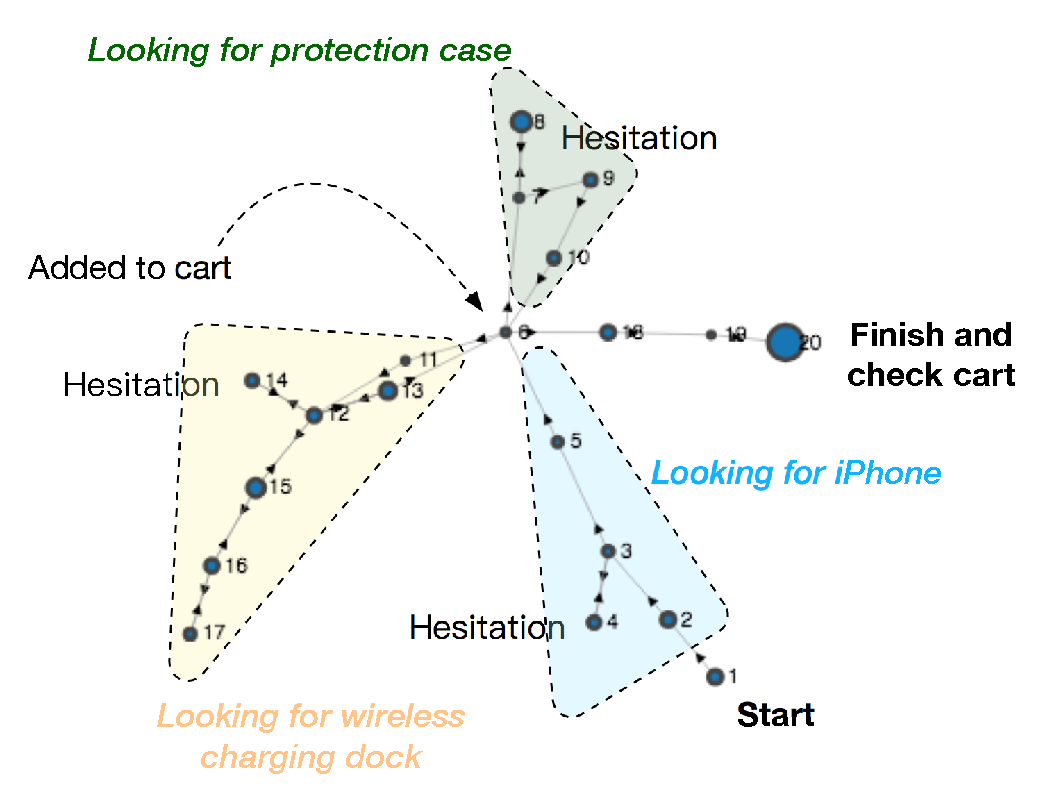
\includegraphics[width=0.55\textwidth]{figures/vis-goal1}
    \caption{Patterns of cluster and hesitation of an action path. This figure visualizes an action path in
    goal-oriented Amazon's task. The visualized graph can be partitioned into four subgraphs
    and three of them are cluster pattern that is a representing of different shopping intent, 
    which is exactly as same as the task design. Further, each cluster contains a hesitation pattern
    as labeled in the figure, for instance, node labeled with 4, 8, 14 are hesitation. 
    Besides, the number of a node is a representative of chronological serial number of user actions.}
    \label{fig:vis-goal1}
\end{figure}

\paragraph{Pattern of ``hesitation''}
Beyound the cluster pattern, we also observes ``hesitation'' pattern in goal-oriented tasks
where a short child path branch from its parent node in each intent cluster, e.g. node
4, 8, 14 in Figure \ref{fig:vis-goal1} and node 5, 16 in Figure \ref{fig:vis-goal2},
which suggests ``hesitation'' is a pattern that more often appears in goal-oriented task
within a ``cluster''. Formally, \emph{a pattern is called ``hesitation'' if and only if it
is a acyclic list and not in a star that joint with a cluster or a ring and the number of its nodes is less than any 
of existed cluster.}

\begin{figure}[H]
    \centering
    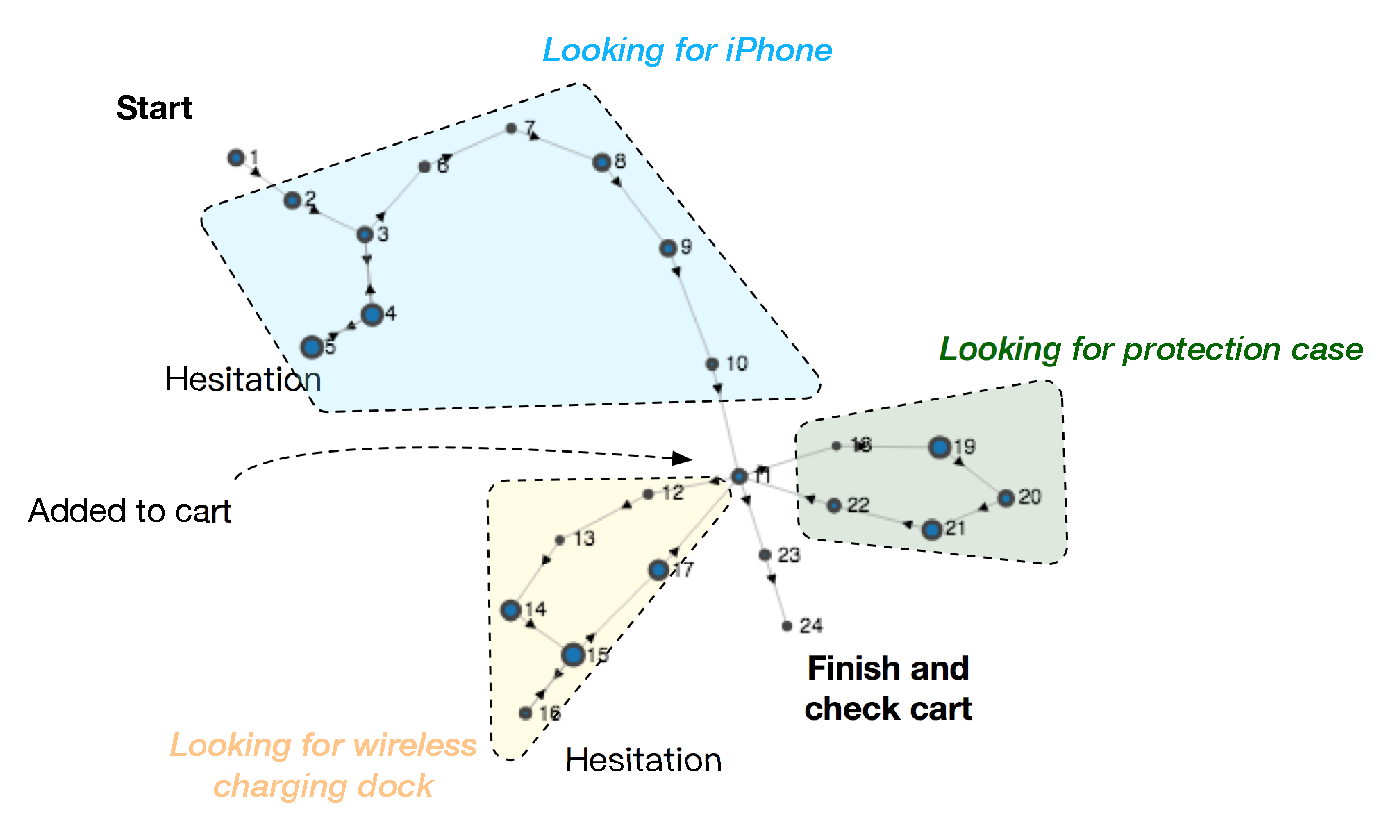
\includegraphics[width=0.55\textwidth]{figures/vis-goal2}
    \caption{Patterns of cluster and hesitation of an action path. This figure visualizes an action path in
    goal-oriented Amazon's task. The visualized graph can be partitioned into four subgraphs
    and three of them are cluster pattern that is a representing of different shopping intent, 
    which is exactly as same as the task design. Further, two of the clusters contain a hesitation pattern
    as labeled in the figure, for instance, node labeled with 5, 16 are hesitation. 
    Besides, the number of a node
    is a representative of chronological serial number of user actions.}
    \label{fig:vis-goal2}
\end{figure}

\paragraph{Pattern of ``ring'' and ``star''}
Similarly, in fuzzy and exploring task, we observed two common pattern ``ring'' and ``star''
pattern is more often to appear in fuzzy and exploring tasks.
Formally, \emph{a pattern is called ``ring'' if and only if it is a list without connect to a cluster
and starting node is not joint with ending node; a pattern is called ``star'' if and only if 
it is a spanning tree of an action path that a non-leaf node contains more than one child.}

Figure \ref{fig:vis-fuzzy-explore1} illustrates an action path of Amazon's fuzzy task (purple nodes)
and an action path of Dribbble's exploring task (orange nodes), both from same participants.
One can observe ``ring'' and ``star'' patterns in the figure as highlighted through 
gray area surrounded by dashed line.

\begin{figure}[H]
    \centering
    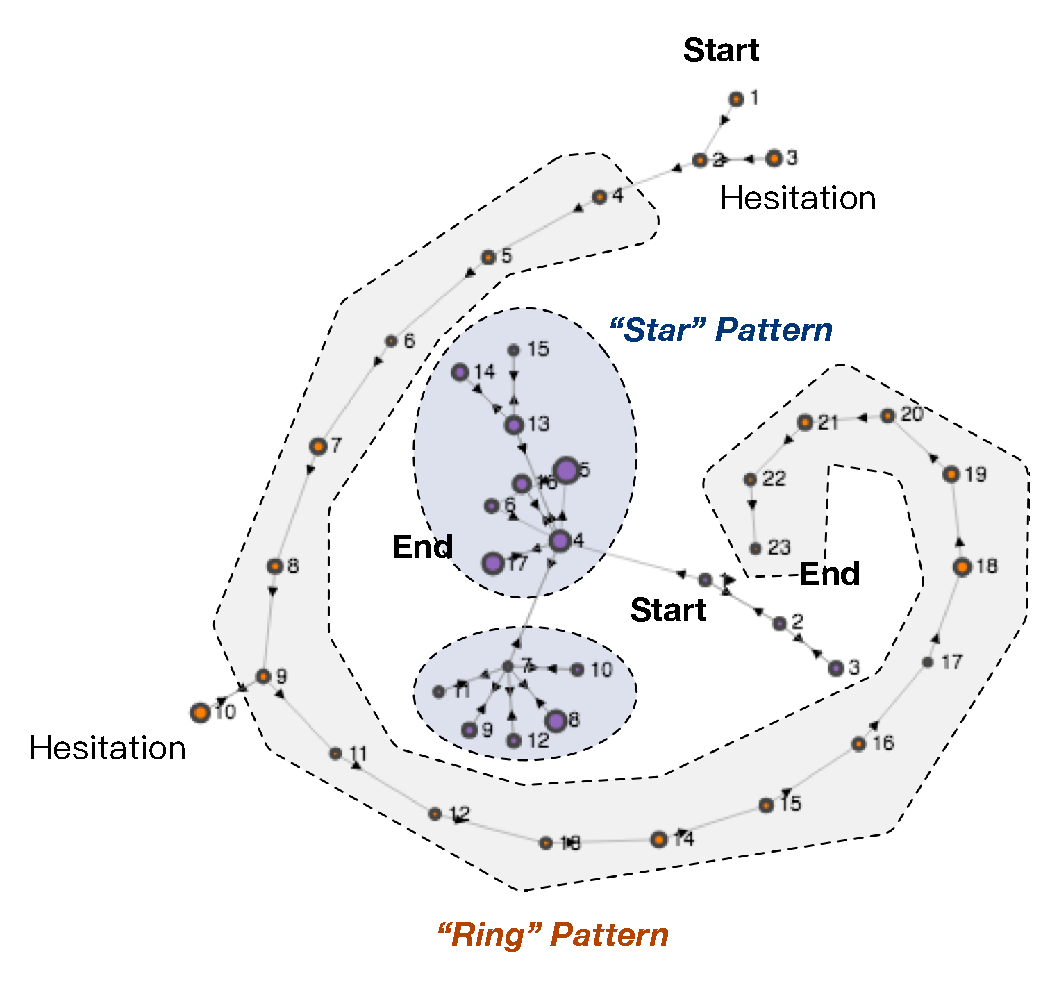
\includegraphics[width=0.55\textwidth]{figures/vis-patterns1}
    \caption{Patterns of ring and star of an action path. The figure visualizes an action path in
    Amazon's fuzzy browsing task (purple nodes) and Dribbble's exploring tasks (orange nodes). 
    The visualized action path of exploring task is an linked list with few hesitations (node 3 and 10).
    The action path of fuzzy task contains two star patterns (roots are 4 and 7).
    As same as other visualizations, the number of a node
    is a representative of chronological serial number of user actions.}
    \label{fig:vis-fuzzy-explore1}
\end{figure}

Similarly, as one more illustration, Figure \ref{fig:vis-fuzzy-explore2} gives action paths 
in same tasks but from another participant that the purple nodes represents actions in Amazon's fuzzy task action path
and orange nodes represents actions in Dribbble's exploring task action path.

In addition, even though we observed that the number of star pattern is more often to appear
in fuzzy tasks and ring pattern is more often to appear in exploring tasks.
We argue that this is because in fuzzy tasks, participants are able to identify the
information uses, therefore the star pattern is more often to appear since it produces many backtracking
behavior and causes the ``differentiating'' activity. However, in the exploring task,
there is no explicit information uses described the exploring task, therefore participants
keep exploring deeper and deeper from the starting page without backtracking, the star pattern
appears when participant has multiple interests on different pages that referred from the same page.

\begin{figure}[H]
    \centering
    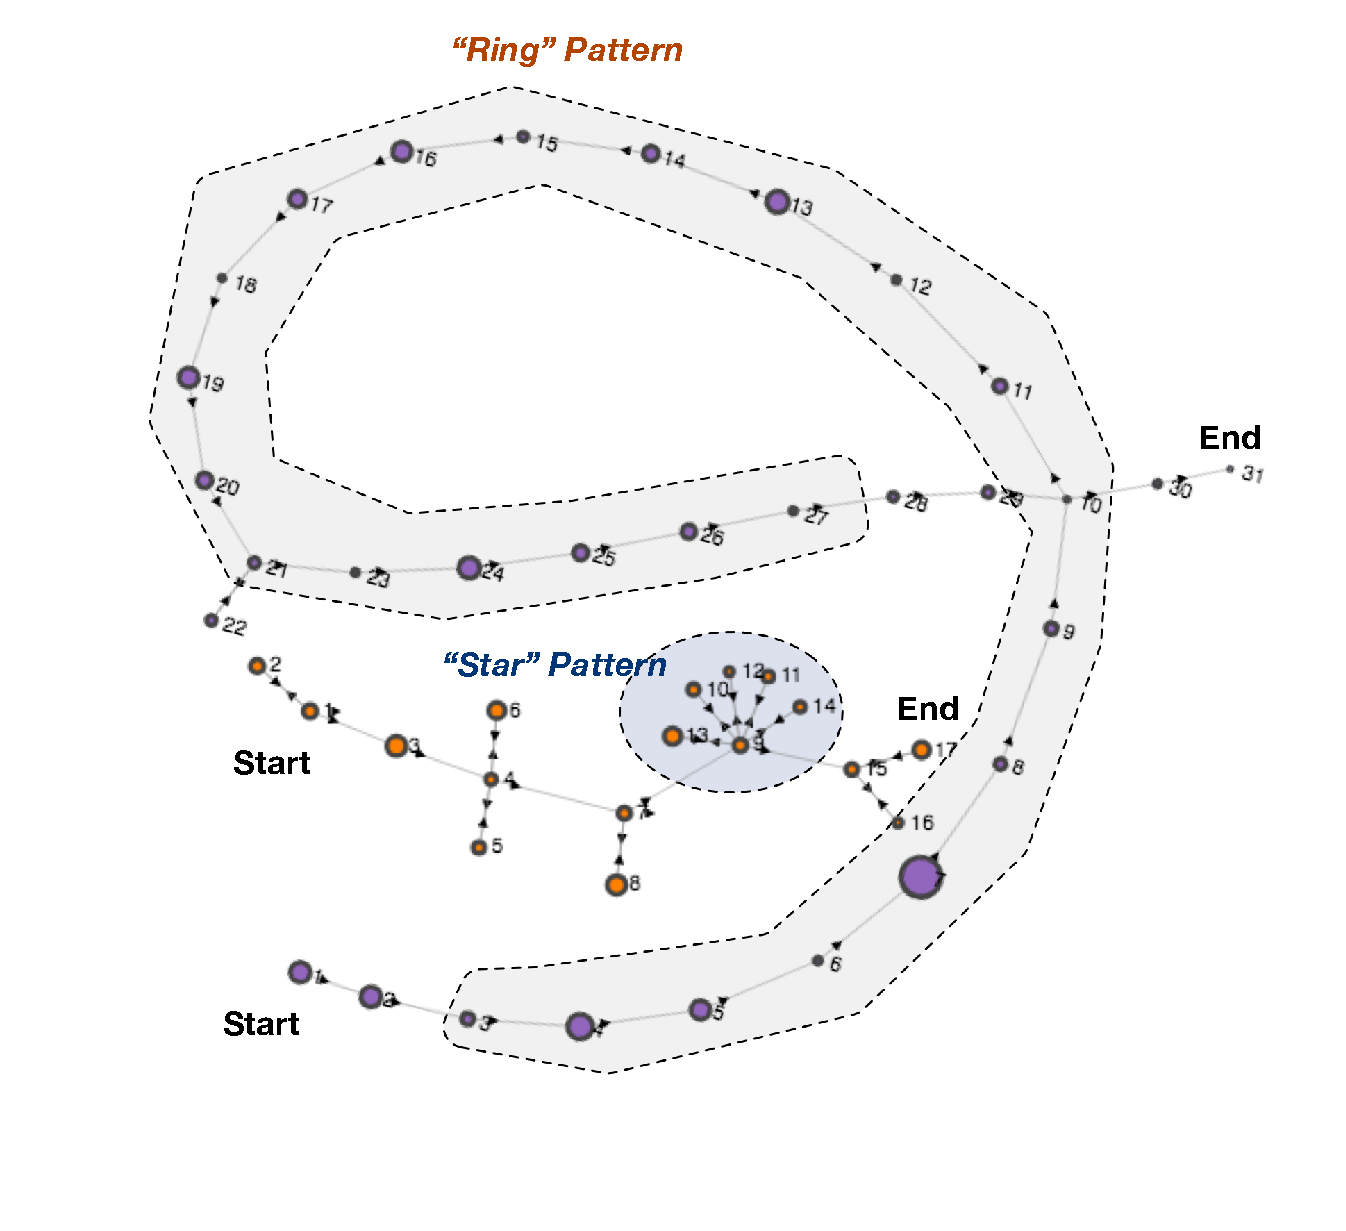
\includegraphics[width=0.55\textwidth]{figures/vis-patterns2}
    \caption{Patterns of ring and star of an action path. The figure visualizes an action path
    of a different participant in
    Amazon's fuzzy browsing task (purple nodes) and Dribbble's exploring tasks (orange nodes). 
    The visualized action path of exploring task contains a star pattern where root is 9.
    The action path of fuzzy task contains a cyclic ring pattern that with a single hesitation
    in node 22.
    As same as other visualizations, the number of a node
    is a representative of chronological serial number of user actions.}
    \label{fig:vis-fuzzy-explore2}
\end{figure}

In summary, we conclude that:

\begin{enumerate}
    \item Goal-oriented browsing behavior contains common patterns of ``cluster'', and each cluster tend to indicate a specific intent;
    \item Fuzzy and exploring behavior two common pattern of ``ring'' and ``star'', however, ring pattern is more often to appear 
          in exploring behavior and star pattern is more often to appear in fuzzy behavior;
    \item Pattern of ``hesitation'' usually attached to a cluster or a ring but not appear in a star.
\end{enumerate}

\subsubsection{Cross user Overlap Patterns}

In the previous discussion we discovered the common patterns that appears in individuals.
Nevertheless, it is still interesting to explore how action paths are manifest to multiple
participants. Fortunately, we observed there are intersections among multiple subjects.

\paragraph{Pattern of ``overlap''}
occurs when we observing action paths on multiple participants. Figure \ref{fig:overlap-example-1}
and \ref{fig:overlap-example-2} are the the action paths visualized for same four participants
in Medium's goal-oriented task and Dribbble's exploring task respectively.
One can define a $n-$overlap ratio is the number of blacken nodes devided by total number of nodes
in the action paths of $n$ participants. Obviously, the maximum number of $4-$overlap ratio
is 100.00\%, and the minimum $4-$overlap ratio is 0.00\%.

\begin{figure}
    \centering
    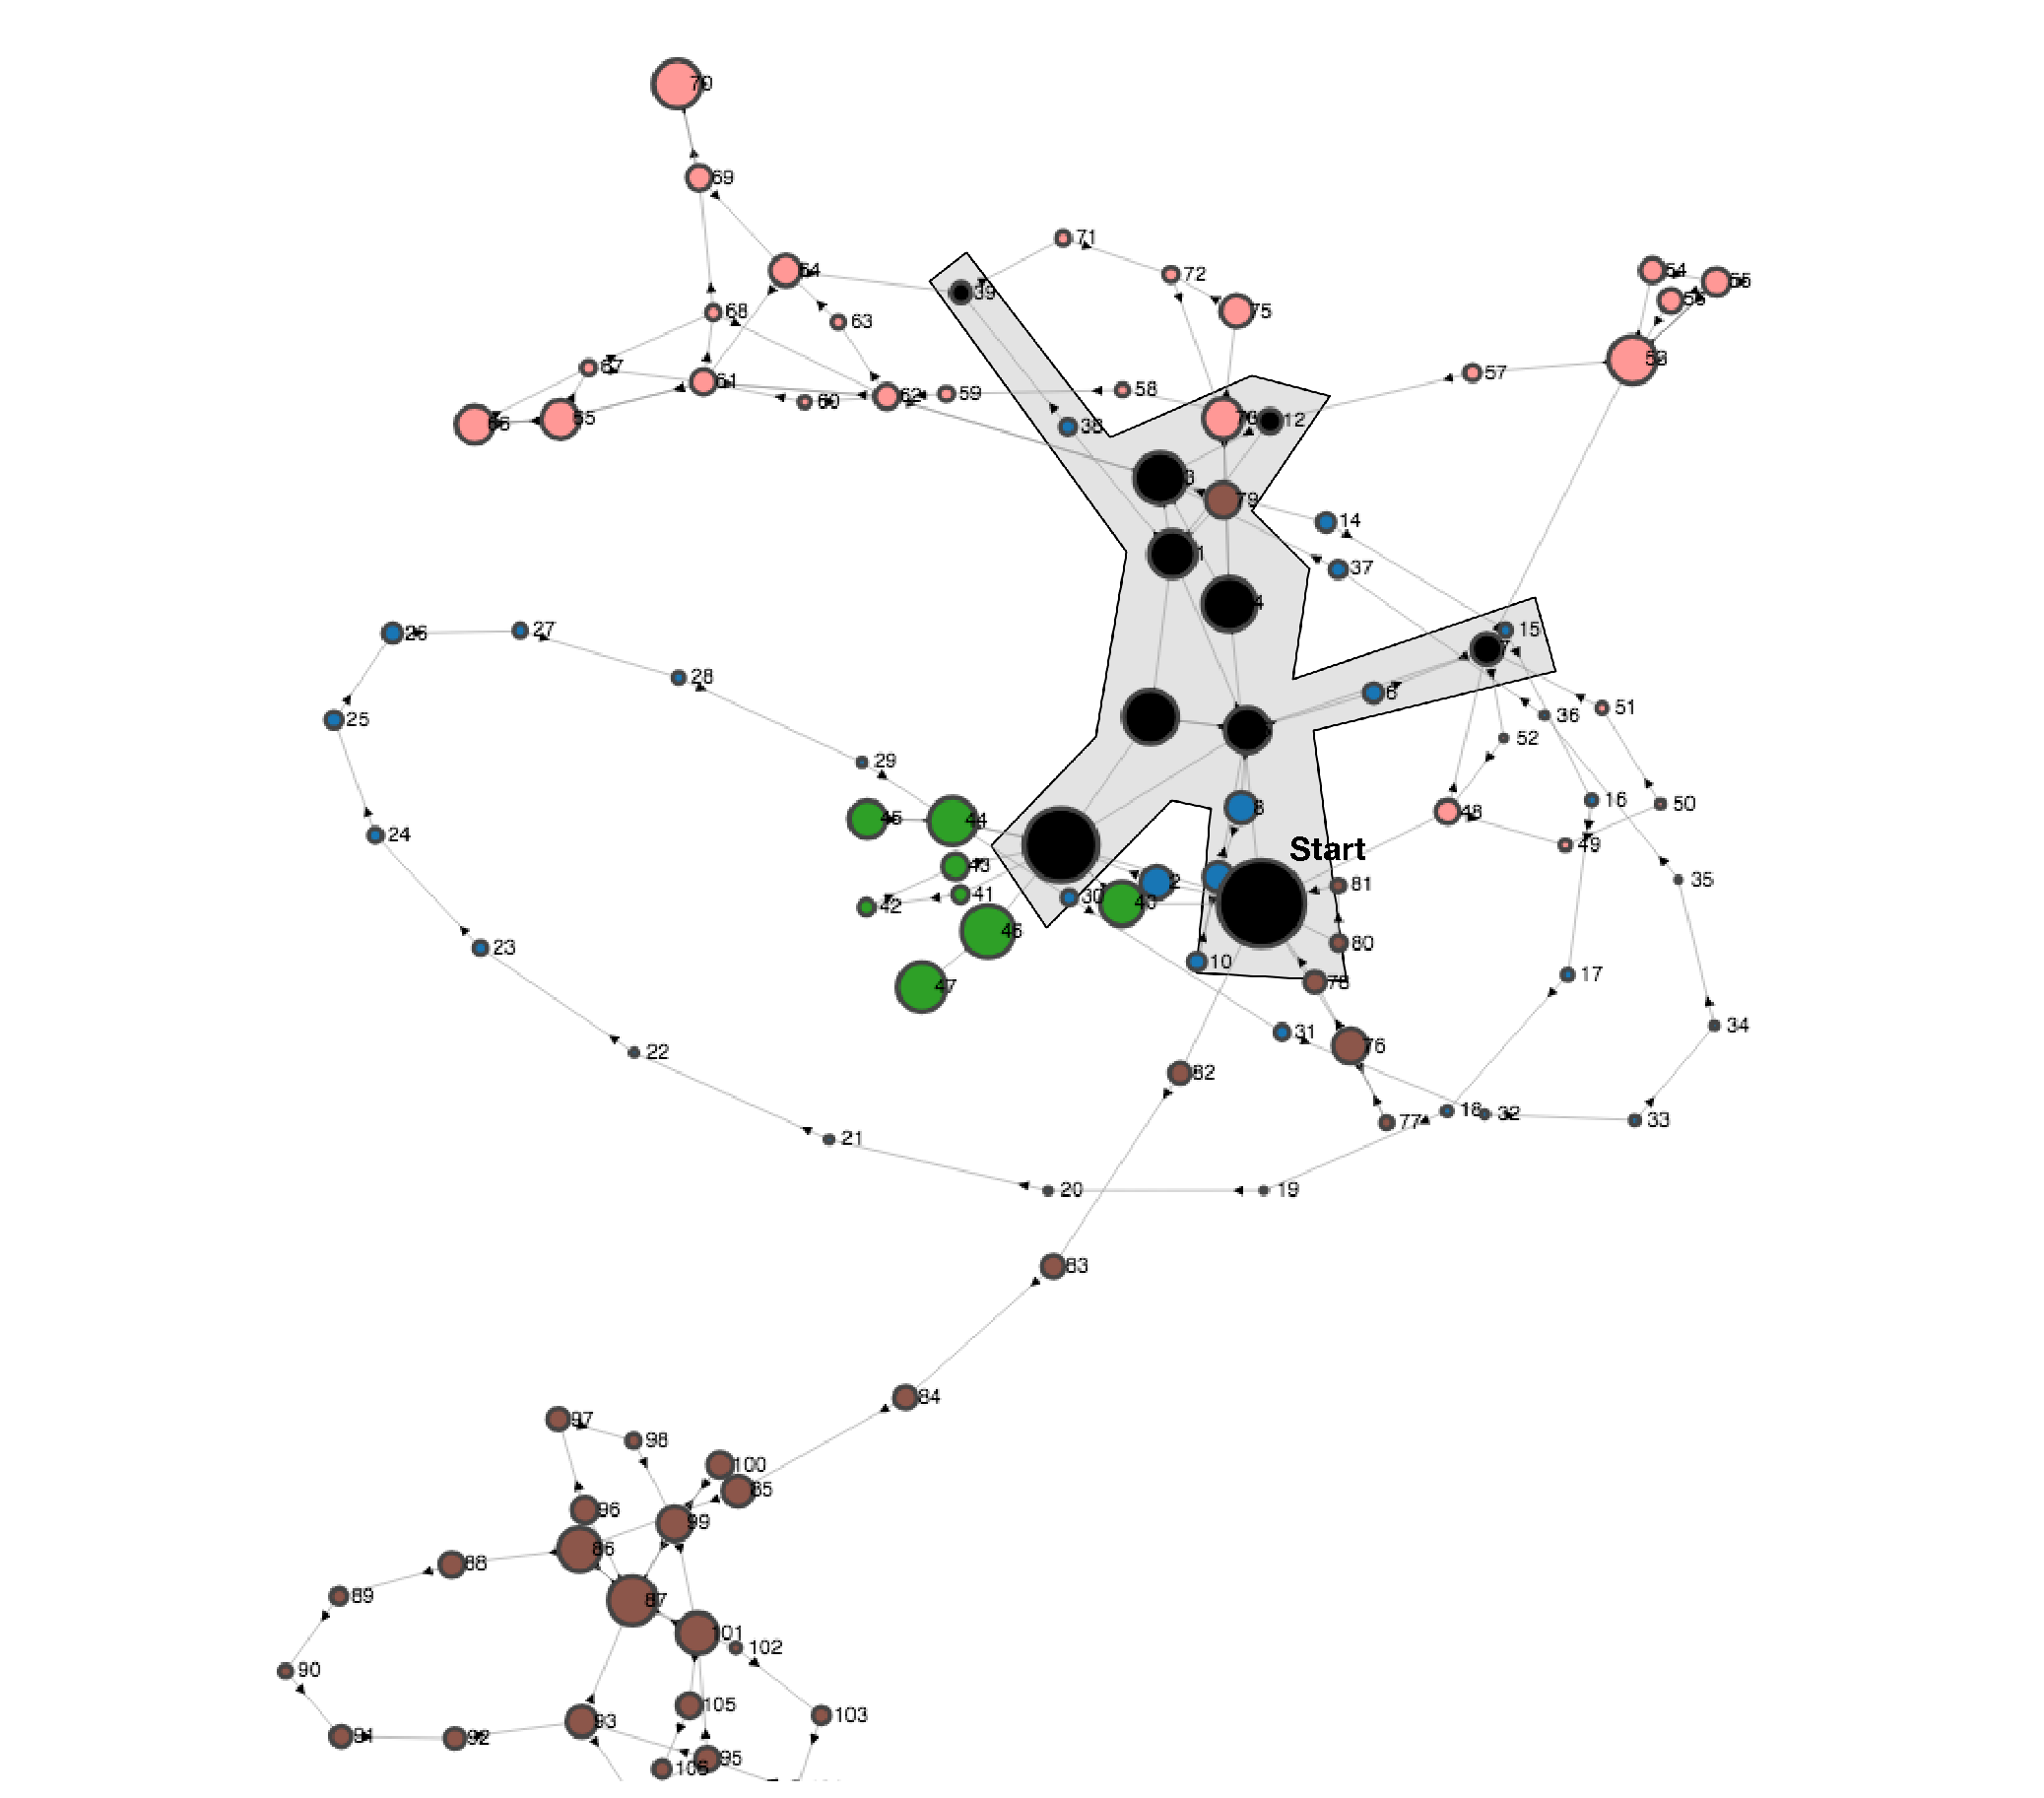
\includegraphics[width=1\textwidth]{figures/overlap1}
    \caption{Example of ``overlap'' pattern in Medium's goal-oriented task: 
    this figure visualize the clickstream intersection 
    of four participants at Medium's goal-oriented task. Each color represents an
    individual clickstream except black nodes, which represents the overlapping of different clickstreams.
    The overlap ratio of this graph is 9.43\%.}
    \label{fig:overlap-example-1}
\end{figure}

However, the highest $4-$overlap ratio and the lowest $4-$overlap ratio we observed from our
dataset is 11.84\% in goal-oriented task and 0.00\% when compare two different tasks, 
therefore we argue that, the browsing behavior tend to be \emph{user-specific} even users has same
goal in a task, however they still share similar overlaps which suggests a \emph{common interests}.

\begin{figure}[H]
    \centering
    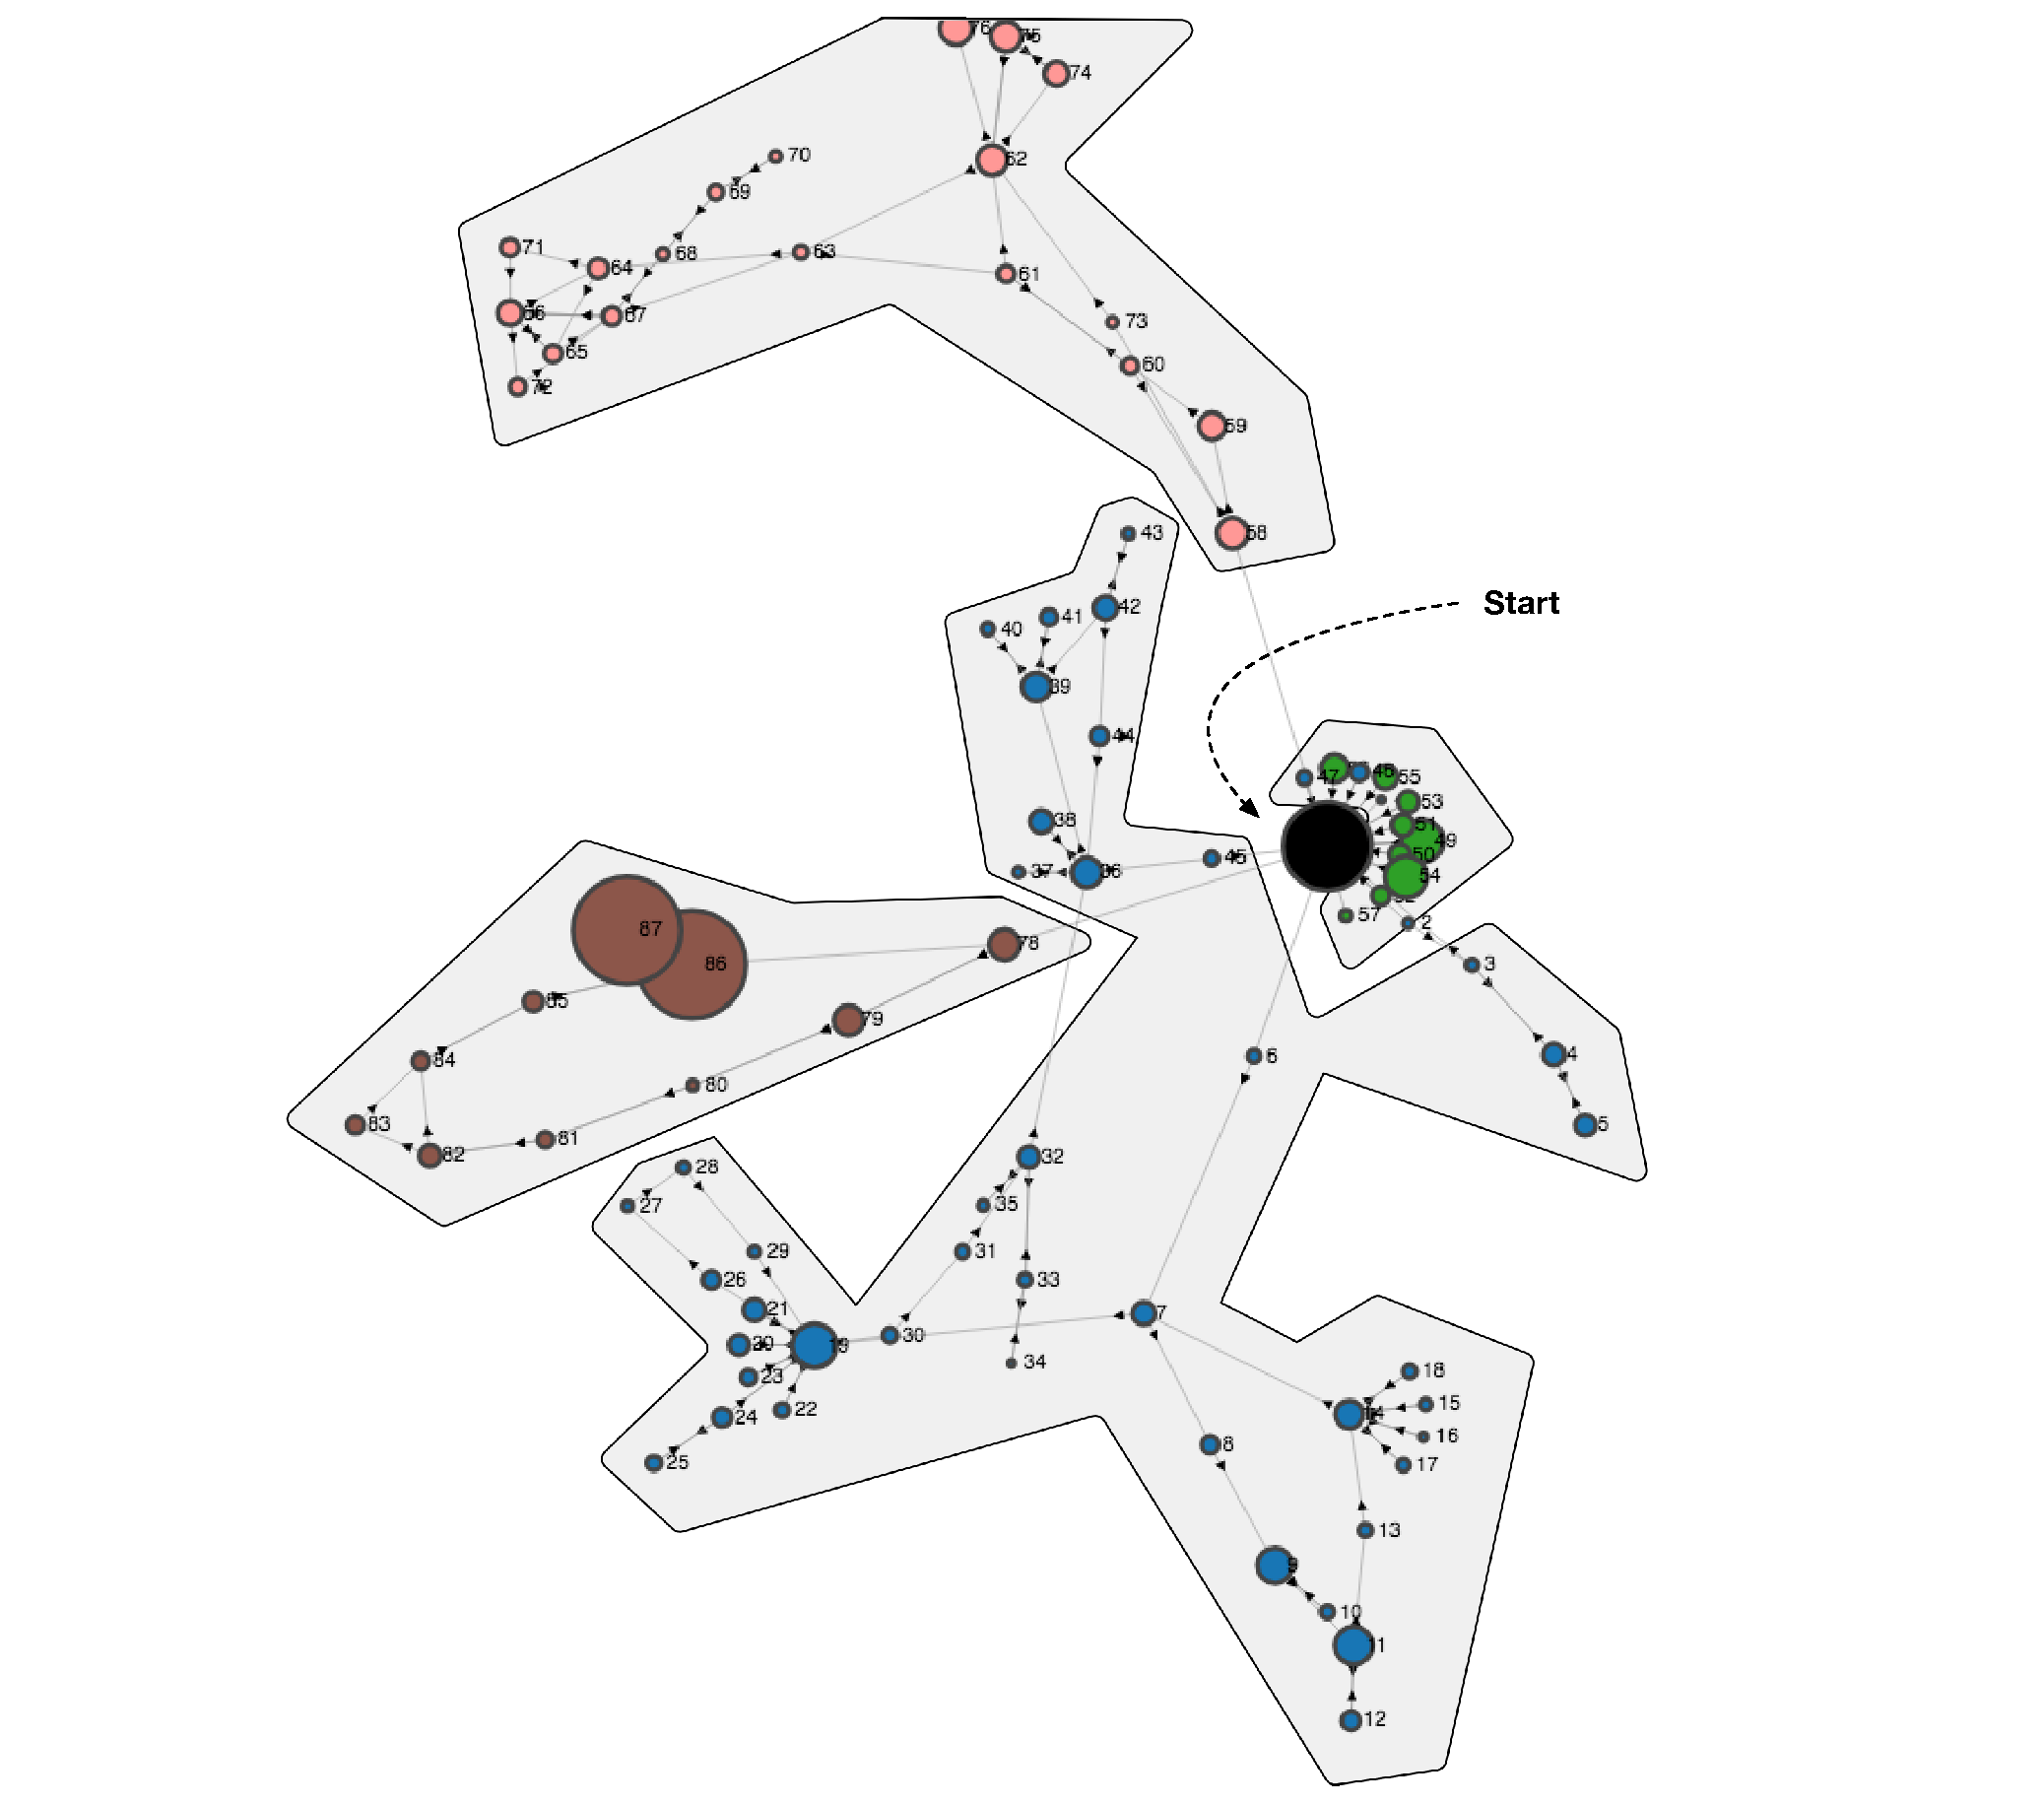
\includegraphics[width=1\textwidth]{figures/overlap2}
    \caption{Example of ``overlap'' pattern in Dribbble's exploring task: \
    this fugure visualize the clickstream intersection
    of four participants at Dribbble's exploring task. Each color represents an
    individual clickstream except blacken nodes, which represents the overlapping of different clickstreams.
    The overlap ratio of this graph is 1.15\%.}
    \label{fig:overlap-example-2}
\end{figure}

In exploring task, the $4-$highest overlap ratio is 1.15\%, which is showed in Figure \ref{fig:overlap-example-2}.
The only common blacken node is the starting page.
This observation suggests us that explroing browsing behavior is highly user-specific.
Therefore, in conclusion, the overlap pattern of action path among multiple users suggests:

\begin{itemize}
    \item Browsing behavior tend to be user specific, however we cannot confirm whether it is 
    user\-specifc because we have an issue with lack of data.
    \item Specifically, in goal-oriented browsing behavior, 
    one can observe common interests between multiple subjects,
    whereas the exploring tasks has no intersection between subjects.
\end{itemize}

\paragraph{Remark} Table \ref{table:ellis-pattern} shows an analysis of all observed patterns
based on Ellis' model, which explains why these patterns exists and how they contributes to our action path model.

\begin{table}
    \small
    \centering
    \caption{Existence of activities from Ellis' Model and information use in the observed patterns}
    \begin{adjustbox}{width=\textwidth}
        \begin{tabular}{ccccccccc}
            \toprule
            \multicolumn{1}{c}{\multirow{2}{*}{\textbf{Behaviors}}}  & \multicolumn{1}{c}{\multirow{2}{*}{\textbf{Information Need}}} & \multicolumn{6}{c}{\textbf{Information Seeking}}                                    & \multicolumn{1}{c}{\multirow{2}{*}{\textbf{Information Use}}} \\ \cline{3-8}
            \multicolumn{1}{c}{}                                     & \multicolumn{1}{c}{}                                  & \textbf{Starting} & \textbf{Chaining} & \textbf{Browsing} & \textbf{Differentiating} & \textbf{Monitoring} & \textbf{Extracting} & \multicolumn{1}{c}{}  \\
            \hline
            cluster    &   observed &       &       &       & Exist & Exist & Exist & Exist \\
            star       &            &       & Exist & Exist & Exist &       &       &       \\
            ring       &            & Exist & Exist &       &       &       &       &       \\
            hesitation &   observed &       & Exist &       & Exist & Exist &       &       \\
            overlap    &   observed &       &       &       &       &       & Exist & Exist \\
            \bottomrule
        \end{tabular}
        \label{table:ellis-pattern}
    \end{adjustbox}
\end{table}

\begin{itemize}
    \item For cluster pattern, as we discussed before, information need can be observed from action path behavior,
    and the differentiating and monitoring contributes to the partitioning characer of the pattern
    and extracting and information then contributes to the short ring and single hesitations
    because the information are specified clearly.
    \item For star pattern, we can neither observe information need from action path nor did the participant uses
    information that find in star pattern. In Ellis' model, chaining, browsing and differentiating contributes to this pattern
    since the deptch from root to leaf node are small.
    \item For ring pattern, we also can neither observe information need or information use, the user explores deeper and deeper
    along the ring until the user exit the browsing session.
    \item For hesitation, it connects to ring and cluster pattern, therefore they have common activities of chaining, differentiating and monitoring.
    However, information from hesitations are not used but one can easily observe the hesitation.
    \item For overlap, we can observe common interests, which indicates inforamtion needs and use, the extracting
    and information use contributes more to represent this behavior.
\end{itemize}

Combining with Table \ref{table:ellis}, cluster pattern and overlap pattern essentially contributes to goal-oriented browsing behavior since they share common
activities in this behavior, star and ring patterns contributes more on fuzzy and exploring tasks since their activities are more close to these browsing behaviors,
besides, as we discussed before, these patterns can not observe a clear information use. 
In addition, the hesitation pattern appears in star, ring and cluster pattern becuase of 
they have common activities, such as chaining and differentiating.

\cleardoublepage
\section{Applications}
\label{ch:app}

This chapter we first introduces a possible application of our proposed model
and how it could benefit user, the proposed design of the application including frontend, backend architecture as well as database that mostly suitable for the data collection.
Then we formalize and discusse the possibility and benefits as a standard Web API for developers.

\subsection{Client Side Browser Plugin}

\begin{figure}[H]
    \centering
    \includegraphics[width=0.7\textwidth]{figures/proactive-noti}
    \caption{TODO:}
    \label{fig:proactive-noti}
\end{figure}


\begin{figure}[H]
    \centering
    \includegraphics[width=0.7\textwidth]{figures/plugin-predicting-result}
    \caption{TODO:}
    \label{fig:plugin-predict}
\end{figure}

\begin{figure}[H]
    \centering
    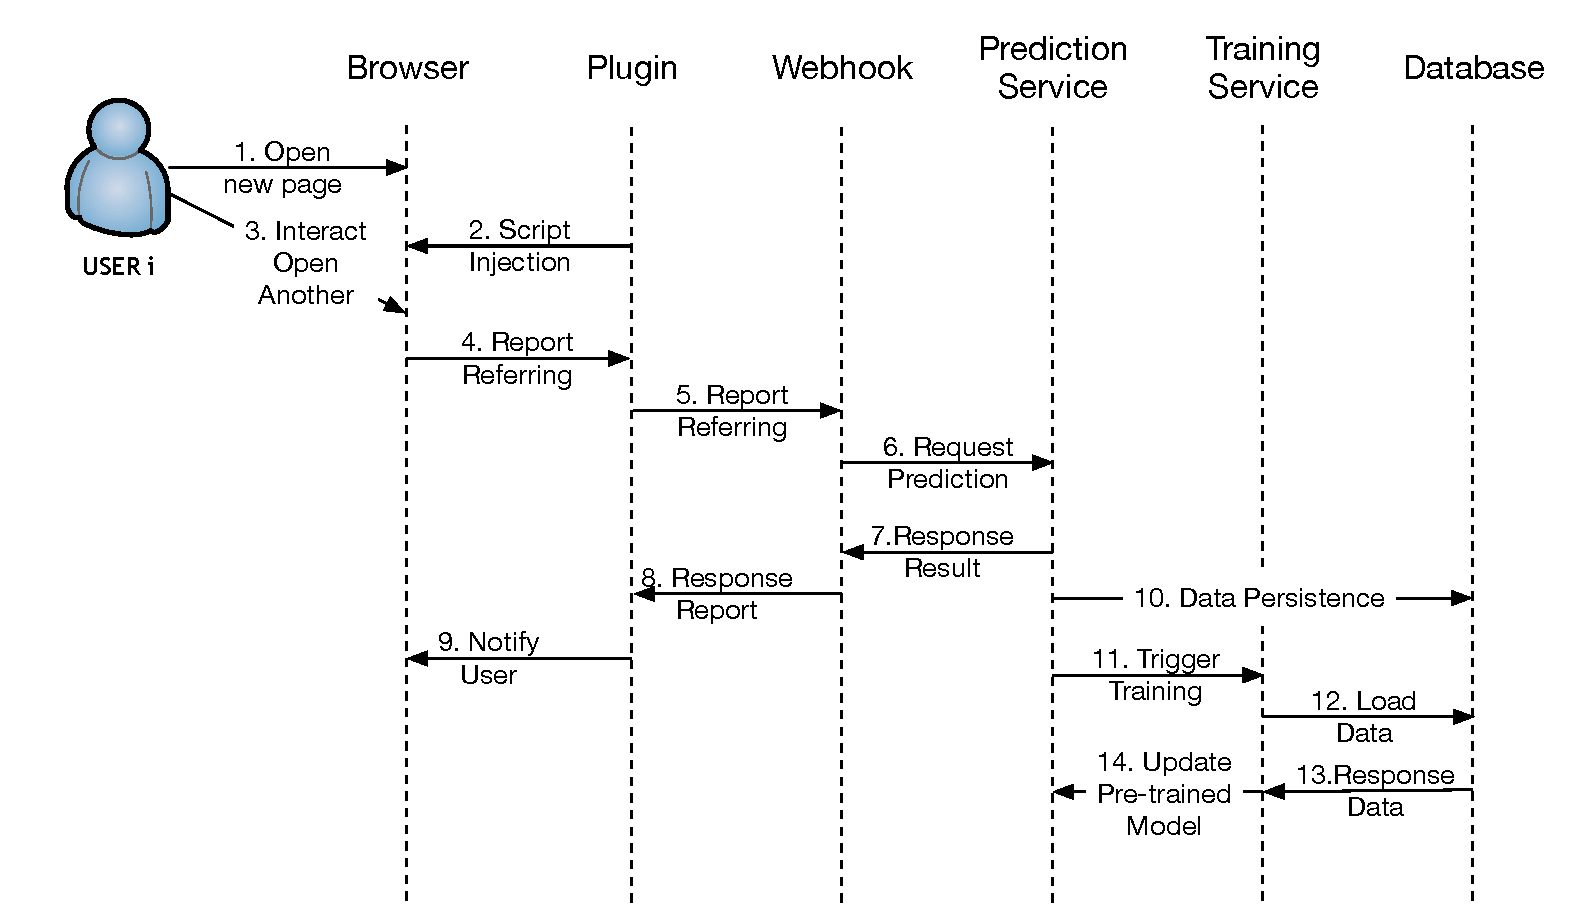
\includegraphics[width=0.7\textwidth]{figures/arch}
    \caption{TODO:}
    \label{fig:arch}
\end{figure}

\subsection{Standard Browser Web APIs}

Web APIs is a generic term used in various fields of development.
Web APIs in a context of web browsers mainly indicates the APIs provided
by browser manufactures to developers that helps web application can even close
to manipulate hardwares, for instance, WebAssembly \cite{w3c2018ws}.

Nowadays, there are experimental standard Web APIs integrates complex features to web developers, e.g. Web Speech APIs \cite{mozilla2019speech}, and only Google Chrome (after version 24) supports. The specification proposal was initiated by Google and according to the source code of Chromium, the APIs are implemented based on the speech recognition service provided by Google Cloud Platform \footnote{\url{https://github.com/chromium/chromium/blob/83928864c18362a4b0f84bad9bee4104f4655430/content/browser/speech/speech\_recognition\_engine.cc\#L35}, last accessed on January 03, 2019}.

\begin{figure}[H]
    \centering
    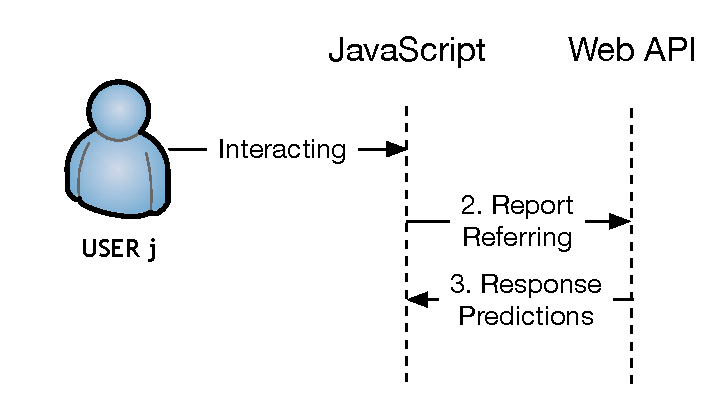
\includegraphics[width=0.4\textwidth]{figures/webapi}
    \caption{TODO:}
    \label{fig:webapi}
\end{figure}

\subsubsection{Communication Protocol}

\subsubsection{Discussion}

\cleardoublepage
\section{Discussion}
\label{ch:discuss}

\epigraph{I think; therefore I am.}{Ren\'e Descartes}

We proposed an action path model that models a sequence of user actions over web browsing
and their decision time of each action simultaneously.
Then we designed and conducted a user study that collects action paths
from participants with different browsing behavior.
We discuss our main findings and the limitations of this work in this chapter.

\subsection{Main Findings}

\paragraph{Clickstream Modeling}

The action path model combines an entire action level clickstream, 
and the stay duration of each action into action path encoder.
Our quantitative results indicate that 
a simply model can easily classify existing three type of browsing
behaviors with 100.00\% of accuracy, i.e. goal-oriented, fuzzy and exploring.
Even further, the model is able to universally (corss-user) predict 3 to 5 future visit 
page with given 95 percent of browsing context.

\paragraph{Browsing Behaviors and Patterns}

We concluded three browsing behaviors based on information behavior theory that describes
three process of web browsing.
Our qualitative analysis 
first interpret the total number of actions 
are more important to contributes the indication of goal-oriented behavior,
and the toal stay duration and completion efficiency are more important to indicate exploring behavior.

Afterwards, we also observed five patterns from client-side clickstream, the ring and star patterns
appears in fuzzy and exploring tasks, ring pattern is more often in exploring task,
and the star pattern is more often in fuzzy task because of differentiating of information use.
A cluster pattern is an indiccation of an individual intent while browsing, and it may connects
few hesitation pattern.
The overlap pattern discovered in the collected action path gains a low overlap ratio,
which suggests action path tend to be a user-specific behavior but reserve a small region as
common interest in goal-oriented browsing behavior.
Next, an analysis based on Ellis' model and Wilson's theory explose the relationship 
of these patterns to the proposed browsing behaviors, and these patterns partially represents a browsing behavior.
Finally, since the model encodes the entire client-side clickstream and stay duration,
the analysis also explains the reason why our model archieves such a good performance.

\subsection{Decisions}

\paragraph{\emph{Why the task difficulty is measured by self-rating scale rather than NASA-TLX?}}


NASA-TLX does not providing more insights than action path to our model.
As we analysed in Section \ref{sec:task-diff}, the major purpose of the measurement of 
task difficulty is to identify inproperate tasks design (i.e. abnormal ourlier) 
rather than the purpose of measuring cognitive load by using NASA-TLX.
Our significant tests to the subjective self-rating scale of task difficulty supports
our argument that these tasks are significant different than one another.

Whether NASA-TLX for cognitive load or self-rating scale for task difficulty is not able to be used in
our machine learning model since they are impossible to be collected from unseen users in bootstrap phase.
Though it is possible to construct a single subjective socre as one of the inputs to the action path model,
the model learns browsing behaviors from all collected data, which means if the model is trained based on 
a dataset with subjective score, then the dataset is biased by these scores and eventually reduces the 
generalization ability in a user-independent context.

\paragraph{\emph{Why leave-one-subject-out cross validation (LosoCV) is not applied in classification task?}}


LosoCV is not necessary in our case. Research in a context of HCI performs a special LosoCV
for a purpose of claiming a model is tested in which it has not seen any unseened user data before,
and arguing this evaluation is a representative of bootstrapping performance of a model.
However, this is an unfortunately inappropriate approach for model performance justification.
LosoSV has been researched many years, statistical research \cite{xu2012asymptotic} proves 
that LosoSV is asymptotically equivalent to k-Fold cross validation, which verifies 
a traditional wisdom that the performance of 
a model that evaluated by LosoCV tend to worth than k-Fold cross validation becuase
LosoCV increases the variance of generalization error \cite{bengio2004no}. Therefore, Gao et al. uses 
model averaging technique (ensemble multiple models that trained through LosoCV when 
leave different subjects) developed a novel regularization technique \cite{gao2016139} 
to help a model generalize better.
Intuitively, when a model that intend to work in a user independent case, 
we are only interested in how well a model could fit universally, 
and how the performance could be changed when a model with fixed architecture applied to more subjects.
More precisely, one can observe that LosoCV is essentially trained on a partial of dataset, 
which is a biased dataset to the training process of the model. Therefore, when we use 
the best model that gains minimum generalization bound is nothing else but a biased learning 
with a part of subjects.
This is not claiming that LosoCV is unnecessary in any cases, the theoretical insights indicates
that LosoCV is critical when a model must be applied in a security context since 
LosoCV provides how well could a model interpret highly correlated clusters 
to individual users and how good of a model could defense an unseened attacker.

For bootstrapping, it is completely non-interests and trivial to the industrial 
becuase the bootstrap in a context of recommending (our application) is valueable if and only if
users do not leave the platform after their first arrival. Therefore, one can solve
the bootstrapping by giving mainstream selection and mainstream preferences, then provide
personalized recommendations after collecting a minimum required dataset since 
collecting data becomes faily easy when a user continuously using a platform.

\paragraph{\emph{Why the experiment is designed under three aggregated browsing behavior instead of
using the existing concluded four or more information seeking behavioris?}}


The main reason of aggregating existing information seeking behaviors is to simplify the 
classification process and expand tasks design scope.


\subsection{Limitations and Future Works}

\paragraph{Lack of data} 
This thesis has a limitation of the lack of data. 
Though we collected 189 clickstreams from 21 subjects, however, 
comparing to the baseline action path model with 90323 parameters in Chapter \ref{ch:eval},
the dataset is still an tiny dataset for the training and learning task.
Moreover, the validation loss (in Figure \ref{fig:class-loss}) suggests our model remains large capacity to learn more
categories of browsing behavior, and prediction performance may be improved
via reparematrization (in Figure \ref{fig:loss}), 
it is still very interesting to see the performance of our model on a large dataset,
and how the this model can adapts to more informations on the web, such as the topic of 
a page, and interpret more detail with attention mechanism.

\paragraph{Data collection}
Our work simulates three proposed browsing behavior through carefully designed browsing tasks.
This method only limit to a small group of users, which is not an appropariate apparoch for
a large dataset collection.
We planed to conducting a field study that install a clickstream collector while a week, 
however there are only two subjects after our lab study
are willing to participate to the field study.

\paragraph{Reinforcement learning appraoch}
As described in Chapter \ref{ch:model}, the dataset that applies to our action path model
is an action-level dataset, which means the sequence of URLs are essentially an series of 
user actions. This could inspire us to use reinforcement learning appraoch to train
an agent that could explore and learn the environment of the web. Eventually,
the agent will be able to learn and optimize the experience of browsing on the web,
which implicitlly solves the problem of data collection and the lack of supervised data.

\paragraph{Privacy}
This work monitors an action level of clickstream, which stores all browsing history of an
individual person on a thirdparty databases, and hence brings a trust and privacy issue of
the application. We positively argue that this is an trust issue between users and service providers.
As we discussed in Chapter \ref{ch:app}, browser providers collect the data anonymously,
and users use the browser because of trusts, then world wide web consortium formalizes
a standardized web API to developers for using this information, and as a browser user can
either authorize developers to use this API or give an explicit rejection.

\paragraph{Proactive serving} 
We are in the era that intellegent system surrounding us. The way we interact with intellegent system
is not as nature as we interact with other people. 
Communications or interactions between humans in a context does not require any trigger word,
and a person can brush out a needs or reacts to another immediately.
The action path prediction gives an working example that shows proactive serving is possible
if we monitors the environment of web browsing. Therefore, it is interesting to study
how this feature could be used by a user and how users reacts to the elimination of interaction trigger
of an intellegent system.

\cleardoublepage
\section{Conclusions}
\label{ch:final}

\subsection{Summary}

% 1. what has been done

This thesis proposed an action path model that describes client-side user clickstream.
To justify our model, we designed nine browsing tasks for three qualitatively
discussed browsing behavior based on the theory of information behavior, then 
held a user study for these tasks that simulates the behaviors. 
Afterwards, we applied the collected data from user study to our action path model and
analysed the model performance to these data with comparison to traditional machine 
learning approach.
Subsequently, we also visualized these data and closely discovered the common, 
individual and intersection patterns among client-side clickstream.
As an application show case, we illustrated a browser plugin that monitors client-side 
user clickstream to predict future movements of web browsing and discussed the benifits of this plugin.
Futhermore, we presented a generic architecture communication flow and architecture of the plugin, 
as well as the possibilities of standardize the plugin feature as browser Web APIs to other developers.

% 2. what are the findings

Our finding indicates the completion difficulty in different type of tasks are significant different,
especially the difficulty of fuzzy task is significant difficult than goal-oriented task,
and the goal-oriented task is also significant difficult than exploring task.
For completion efficiency, length of client-side clickstream and total duration of the clickstream

% 3. emphasize the importance >> place to large context
Our findings are generic and subservience. The model can not only be use on desktop but
also can be implemented in a mobilephone, or even a outside the context of web browsing. 
Similar to other user behavior data, client-side user clickstream or user actions 
directly indicates movements of a user and how they making decisions. Understanding, 
interpreting and predicting these data not only improves the user experience when doing
web browsing, but also useful to help users reducing useless browsing, better controls 
and manages their time. Moreover, by standardize the data processing process can formalize
the feature to developers, and then help them using the behavior predictions to
improve their product user experience.

% 4. summarize / conclude
Traditional server collected clickstream data has been proved its high value in many fields. With our work we exposit the value one-step forward, and contributes to models and approaches that hope to bring ponderable research to the community.


\cleardoublepage
\input{contents/ch09-appendix}

\part*{Bibliography}

\addcontentsline{toc}{part}{Bibliography}
\nocite{*}
\bibliographystyle{plain}
\bibliography{literature/list}
\end{document}